\documentclass[lettersize,journal]{IEEEtran}

\usepackage[export]{adjustbox} % Ajustes gráficos
\usepackage{amsmath,amsfonts}
\usepackage{amssymb}         % Símbolos adicionales
\usepackage{algorithm}
\usepackage{algorithmic}
\usepackage{array}
\usepackage{booktabs}        % <-- NECESARIO para \toprule \midrule \bottomrule
\usepackage{cite}
\usepackage{fontawesome}     % Íconos FontAwesome (opcional)
% --- Soporte de caracteres extendidos (necesario para \DJ, \dj en .bib) ---
\usepackage[T1]{fontenc}
\usepackage{graphicx}
\usepackage[hidelinks]{hyperref}
\usepackage{microtype}       % Mejoras tipográficas
\usepackage{multirow}        % <-- NECESARIO para \multirow (ver más abajo)
\usepackage{multicol}        % <-- NECESARIO para \multirow (ver más abajo)
%%\usepackage{subcaption}      % Subfiguras
\usepackage{stfloats}
\usepackage[caption=false,font=normalsize,labelfont=sf,textfont=sf]{subfig}
\usepackage{tabularx}        % Tablas anchas
\usepackage{textcomp}
\usepackage{tikz}            % Dibujos vectoriales
\usepackage{url}             % URLs automáticas
\usepackage{verbatim}
\usepackage{xcolor}          % Colores
\hyphenation{op-tical net-works semi-conduc-tor IEEE-Xplore}
% updated with editorial comments 8/9/2021

\graphicspath{{figs/}}

\begin{document}
    \title{AI-Driven Inclusive Mobile Messaging System for Users with Visual, Hearing, or Speech Impairments}
    
    \author{
        Gleiston Guerrero-Ulloa, Jhon Leturne, and Efraín Díaz-Macías,~\IEEEmembership{State Technical University of Quevedo, Ecuador},\\
        Miguel J. Hornos and Carlos Rodríguez-Domínguez,~\IEEEmembership{University of Granada, Spain}
        \thanks{Manuscript received October XX, 2020; revised Month XX, 2021. This work was supported in part by the Universidad Técnica Estatal de Quevedo, Ecuador, and the University of Granada, Spain. Corresponding author: G. Guerrero-Ulloa (email: gguerrero@uteq.edu.ec).}
    }
    
    \markboth{IEEE Transactions on Human-Machine Systems,~Vol.~XX, No.~X, Month~202X}%
    {Guerrero-Ulloa \MakeLowercase{\textit{et al.}}: AI-Driven Inclusive Mobile Messaging System}
    
    \maketitle
    
    \begin{abstract}
        Este artículo presenta una aplicación móvil inclusiva diseñada para mejorar la accesibilidad y la participación social de personas con discapacidades visuales, auditivas o del habla. El sistema realiza la conversión automática y multimodal de mensajes entre texto, voz e imágenes, adaptándose en tiempo real al perfil de accesibilidad de cada usuario. Todo el procesamiento se ejecuta localmente mediante módulos ligeros de inteligencia artificial —Whisper para voz a texto, Pyttsx3 y Edge-TTS para texto a voz, y BLIP para descripción de imágenes—, garantizando la privacidad de los datos y una baja latencia. El desarrollo se llevó a cabo bajo la metodología TDDM4IoTS, que combina enfoques de Model-Driven Engineering y Test-Driven Development para favorecer la refinación iterativa y la escalabilidad modular. La interfaz de usuario cumple con los estándares WCAG 2.1, asegurando contraste adecuado, tipografía legible y compatibilidad con tecnologías de asistencia como TalkBack y VoiceOver. Una evaluación de usabilidad, aplicada a usuarios con discapacidades auditivas y visuales bajo el modelo TAM, evidenció una mejora del 37\% en la eficiencia comunicativa y en la satisfacción general frente a aplicaciones convencionales. El cifrado de extremo a extremo garantiza la seguridad de las transmisiones. Los resultados confirman que la interacción multimodal basada en IA local puede reducir las brechas de accesibilidad en la mensajería móvil y fortalecer la simbiosis adaptativa entre humanos y máquinas en entornos digitales inclusivos.
    \end{abstract}

    \begin{IEEEkeywords}
        Inclusive communication, mobile accessibility, human–machine interaction, assistive technologies, speech processing, on-device artificial intelligence, usability evaluation, accessibility standards.
    \end{IEEEkeywords}

    \section{Introducción}
        \IEEEPARstart{L}{os} avances tecnológicos se han consolidado como un pilar fundamental para mejorar la calidad de vida de las personas con discapacidades. No obstante, la accesibilidad sigue siendo limitada debido a barreras persistentes en el diseño de entornos digitales y sistemas de interacción humano–máquina \cite{Manirajee2024}. En particular, el uso de tecnologías móviles y aplicaciones de mensajería ha fortalecido la comunicación y la autonomía de numerosos usuarios \cite{Shezi2020}; sin embargo, las personas con discapacidades auditivas o del habla continúan enfrentando importantes restricciones de interacción \cite{Seebun2020}. Dado que los teléfonos inteligentes se han convertido en las principales herramientas de comunicación, desarrollar interfaces inclusivas y adaptativas que integren múltiples modalidades sensoriales constituye un desafío crucial dentro del diseño de sistemas humano–máquina \cite{Kaur2020}.
        
        Según la Organización Mundial de la Salud (OMS), aproximadamente el 5\% de la población mundial presenta algún tipo de discapacidad auditiva o del habla, lo que limita su capacidad para comunicarse de manera efectiva mediante aplicaciones móviles convencionales \cite{Chhajed2021}. De igual forma, las personas con discapacidad visual encuentran dificultades al interactuar con elementos de interfaz no perceptibles por los lectores de pantalla o las herramientas de asistencia \cite{Khan2020}. Si bien los dispositivos actuales integran funciones de accesibilidad, como la lectura de pantalla o el reconocimiento de voz, estas soluciones continúan siendo insuficientes para cubrir la diversidad de necesidades entre distintos grupos de usuarios \cite{Kaur2020}.
        
        En el contexto ecuatoriano, la discapacidad auditiva representa aproximadamente el 50.30\% de los casos registrados, seguida de la discapacidad visual con un 45.39\%, mientras que los problemas del habla afectan al 4.31\% de la población \cite{CONADIS2024}. La mayoría de las personas afectadas son adultos mayores, lo que resalta la importancia de diseñar aplicaciones intuitivas, de bajo tiempo de aprendizaje y accesibles a diferentes edades y condiciones sensoriales \cite{Zaid2023}. Además, se requiere una estrategia de socialización y capacitación que fomente la adopción y el uso sostenido de estas tecnologías \cite{Yeratziotis2022}.
        
        En años recientes, diversas investigaciones han desarrollado aplicaciones web y móviles para facilitar la interacción de usuarios con discapacidades visuales o auditivas. Por ejemplo, Kaur et al.~\cite{Kaur2020} implementaron servicios basados en voz mediante la tecnología TalkBack de Android, mientras que Shezi y Ade-Ibijola~\cite{Shezi2020} diseñaron una herramienta que utiliza reconocimiento de voz para transcribir conversaciones grupales en tiempo real. Asimismo, Guerrero-Ulloa et al.~\cite{GuerreroUlloa2024} desarrollaron BellChat, una aplicación web que convierte mensajes de texto a voz y viceversa para usuarios con discapacidades auditivas o visuales. No obstante, estas propuestas suelen enfocarse en un solo tipo de discapacidad o dependen de infraestructuras web, lo cual limita su portabilidad y la interacción táctil característica de los dispositivos móviles \cite{Sami2023}.
        
        Motivado por estas limitaciones, este trabajo propone una aplicación móvil inclusiva de mensajería que permite la comunicación entre personas con discapacidades visuales, auditivas o del habla, y usuarios sin discapacidades. El sistema adapta dinámicamente el formato de los mensajes —texto, audio o visual— en función de la configuración de accesibilidad de cada usuario. Por ejemplo, un mensaje enviado a una persona con discapacidad visual se convierte automáticamente en audio, mientras que un mensaje dirigido a un usuario con discapacidad auditiva se muestra en formato textual. En el caso de las personas con discapacidad del habla, la aplicación ajusta la modalidad de interacción según sus preferencias, permitiendo una comunicación bidireccional plena.
        
        El sistema propuesto integra conversión multimodal automatizada, procesamiento en tiempo real y transmisión segura mediante cifrado de extremo a extremo, garantizando así una comunicación accesible, privada y confiable. La combinación de ingeniería de accesibilidad, interfaces adaptativas e inteligencia artificial local contribuye al avance de los sistemas inclusivos dentro del campo de los sistemas humano–máquina.
        
        Las principales contribuciones de este trabajo son las siguientes:
        \begin{enumerate}
            \item Una arquitectura de aplicación móvil que permite la conversión dinámica entre texto, audio e imagen para garantizar la accesibilidad entre distintos tipos de discapacidad;
            \item Un marco de comunicación inclusiva que soporta el intercambio de mensajes cifrados en tiempo real;
            \item Un diseño de interfaz optimizado para la accesibilidad y la facilidad de uso entre adultos mayores con discapacidades sensoriales; y
            \item Una validación comparativa de la accesibilidad respecto a sistemas web y móviles existentes.
        \end{enumerate}
        
        El resto de este artículo se organiza de la siguiente manera: la Sección~II presenta los trabajos relacionados sobre sistemas de comunicación accesibles. La Sección~III describe el diseño y la implementación de la aplicación propuesta. La Sección~IV expone la metodología de evaluación y la Sección~V analiza los resultados e implicaciones. Finalmente, la Sección~VI concluye este trabajo y propone líneas futuras de investigación en sistemas humano–máquina inclusivos.
        
    \section{Trabajos relacionados}
        En los últimos años, la investigación en accesibilidad digital ha experimentado un crecimiento sustancial, impulsado por la convergencia entre inteligencia artificial, interacción multimodal y diseño centrado en el usuario. Este avance ha dado lugar a múltiples soluciones orientadas a la comunicación inclusiva, tanto en entornos web como móviles, que buscan reducir las barreras que enfrentan las personas con discapacidades sensoriales o del habla. A continuación, se presentan los enfoques más representativos en función de las plataformas tecnológicas empleadas y el tipo de discapacidad abordada.
        
        \subsection{Aplicaciones web inclusivas}
            Diversos estudios han explorado la implementación de aplicaciones web destinadas a mejorar la comunicación y el acceso a la información para personas con discapacidades visuales o auditivas. Guerrero-Ulloa et al.~\cite{GuerreroUlloa2024} desarrollaron \textit{BellChat}, una plataforma que integra servicios de conversión entre texto y voz en tiempo real mediante APIs de reconocimiento de audio y comunicación asincrónica por WebSockets. Su diseño basado en JSF~2.3 y PostgreSQL bajo el patrón MVC garantiza estabilidad y modularidad, aunque su dependencia de entornos de escritorio limita la usabilidad móvil.  
            
            En el ámbito educativo, Bharadwaj et al.~\cite{Bharadwaj2020} propusieron un sistema de evaluación automatizado que permite a estudiantes con discapacidad visual realizar exámenes de forma autónoma mediante síntesis y reconocimiento de voz. De manera complementaria, Matoušek et al.~\cite{Matousek2020} y Cruz et al.~\cite{Cruz2020} abordaron la accesibilidad en plataformas de aprendizaje a través de interfaces auditivas y comandos de voz. Aunque estas propuestas facilitan la interacción con contenido educativo, se centran en tareas unidireccionales y carecen de mecanismos de comunicación interactiva o adaptativa en tiempo real.
            
            Otros autores han dirigido sus esfuerzos hacia la accesibilidad en entornos clínicos y de ocio digital. Buzzi et al.~\cite{Buzzi2024} presentaron \textit{ELSA}, un chatbot médico accesible desarrollado con Flask e impulsado por modelos de lenguaje natural como ChatGPT, orientado a usuarios mayores o con discapacidades cognitivas. Asimismo, Lee et al.~\cite{Lee2021} propusieron \textit{AccessComics}, una herramienta web que permite la lectura adaptada de cómics mediante descripciones visuales generadas automáticamente. Aunque ambos sistemas logran una experiencia más inclusiva, su dependencia de la conectividad constante y la ausencia de procesamiento local representan limitaciones en términos de autonomía, privacidad y latencia.
            
            Finalmente, Erelli et al.~\cite{Erelli2024} y Agnihotri y Kaur~\cite{Agnihotri2023} abordaron la gestión de correo electrónico accesible a través de comandos de voz y retroalimentación auditiva. El primero integró \textit{Whisper} y \textit{GTTS} para transcripción y lectura, mientras que el segundo empleó HTML5 y módulos SMTP con algoritmos de seguridad hash. Ambos sistemas demostraron la viabilidad de la comunicación asistida por voz, aunque restringidos al paradigma tradicional del correo electrónico, sin capacidades de mensajería instantánea o interoperabilidad multimodal.
        
        \subsection{Aplicaciones móviles accesibles}
            El desarrollo de aplicaciones móviles inclusivas se ha consolidado como una tendencia prioritaria en la interacción humano–máquina. La literatura reciente puede agruparse en tres líneas principales: comunicación para usuarios con discapacidades auditivas o del habla, asistencia para personas con discapacidad visual y uso de agentes inteligentes para la mediación conversacional.
        
            \subsubsection{Comunicación para personas con discapacidades auditivas o del habla}
                Seebun et al.~\cite{Seebun2020} presentaron \textit{Let’s Talk}, una aplicación móvil que combina reconocimiento de voz, síntesis de texto a voz y traducción de lenguaje de señas mediante procesamiento de imágenes con OpenCV y algoritmos de soporte vectorial (SVM). De forma paralela, Stefanov et al.~\cite{Stefanov2024} diseñaron una aplicación que traduce texto a gestos animados dentro del chat, implementada con React Native. Por su parte, Shezi y Ade-Ibijola~\cite{Shezi2020}, junto con Yeratziotis et al.~\cite{Yeratziotis2023}, desarrollaron soluciones que incorporan teclados basados en el alfabeto de señas e integración con IBM Watson para conversión de voz a texto. Aunque estos sistemas amplían la inclusión comunicativa, dependen fuertemente de servicios en la nube y carecen de cifrado integral, lo que compromete la privacidad del usuario.
            
            \subsubsection{Aplicaciones para personas con discapacidad visual}
                Caballero et al.~\cite{Caballero2020} propusieron una aplicación de reconocimiento de objetos basada en redes neuronales convolucionales (CNN) que genera descripciones auditivas del entorno, favoreciendo la autonomía de usuarios con discapacidad visual. De manera complementaria, Dognin et al.~\cite{Dognin2021} desarrollaron un sistema de captioning basado en modelos Transformer y reconocimiento óptico de caracteres (OCR), utilizando el conjunto de datos VizWiz capturado por personas con discapacidad visual. Su enfoque fusiona detección de texto y objetos con generación automática de descripciones auditivas mediante la API IBM Watson Text-to-Speech, demostrando el potencial de la inteligencia artificial multimodal para proveer información contextual relevante en tiempo real. 
                
                Asimismo, Norkhalid et al.~\cite{Norkhalid2020} realizaron una revisión de asistentes móviles para personas con discapacidad visual, centrados en clasificación de imágenes mediante TensorFlow y comandos por voz basados en modelos ocultos de Markov (HMM) y redes neuronales artificiales (ANN). Su estudio evidencia el papel de la visión por computadora y la síntesis de voz como herramientas clave para la autonomía y navegación asistida en entornos reales. Polys y Wasi~\cite{Polys2023} extendieron este enfoque hacia la accesibilidad en entornos virtuales tridimensionales, empleando el algoritmo YOLO para detección de objetos y la API Web Speech para interacción por voz. Asimismo, Miguel et al.~\cite{Negrao2021} desarrollaron \textit{SpeechToText}, una herramienta de transcripción de audio mediante reconocimiento automático de voz (ASR) y detección de actividad vocal (VAD). Estos trabajos evidencian avances en percepción asistida, pero no abordan la interacción comunicativa entre múltiples usuarios ni la adaptación contextual de modalidades sensoriales.
                    
            \subsubsection{Aplicaciones con chatbots e inteligencia artificial}
                En el ámbito de la comunicación mediada por agentes conversacionales, Mateos-Sánchez et al.~\cite{MateosSanchez2022} desarrollaron un chatbot móvil para la estimulación cognitiva de personas con discapacidades intelectuales, mientras que Singh et al.~\cite{Singh2024} implementaron un asistente agrícola accesible que integra mensajería por voz y texto en plataformas populares como WhatsApp y Telegram. Si bien ambos casos demuestran el potencial de la inteligencia artificial para la personalización y el soporte contextual, dependen de infraestructuras externas y no incorporan adaptación multimodal en tiempo real.
                
                En una línea de interacción más avanzada, Velasco-Álvarez et al.~\cite{VelascoAlvarez2021} desarrollaron un sistema de interfaz cerebro–computadora (BCI) que permite controlar aplicaciones de mensajería como WhatsApp y Telegram mediante comandos de voz y señales cerebrales. Su integración con el asistente UMA-BCI Speller y Google Assistant posibilita la lectura y envío de mensajes sin interacción manual, ampliando el horizonte de la comunicación asistida hacia entornos neurotecnológicos.
                    
        \subsection{Síntesis y brechas identificadas}
            El análisis de la literatura muestra una evolución significativa hacia la inclusión digital mediante la combinación de procesamiento de voz, visión por computadora e inteligencia artificial. Sin embargo, la mayoría de las soluciones revisadas presentan limitaciones comunes: dependencia de conexión a internet, falta de procesamiento local, cobertura limitada de tipos de discapacidad y ausencia de interoperabilidad multimodal. Estas restricciones evidencian la necesidad de sistemas móviles que integren conversión dinámica entre texto, audio e imagen, con ejecución local y comunicación cifrada de extremo a extremo.  
                
            En este contexto, el sistema propuesto en este trabajo responde a dichas brechas al combinar procesamiento inteligente en dispositivo, adaptación multimodal y seguridad en tiempo real, contribuyendo así al desarrollo de una comunicación verdaderamente inclusiva dentro del campo de los sistemas humano-máquina.
                    
    \section{Materiales y métodos}
    
        En este apartado se describen los materiales y métodos utilizados para el desarrollo de la aplicación móvil inclusiva, detallando los recursos tecnológicos empleados y los procedimientos seguidos para su implementación, integración, despliegue y evaluación funcional.

        \subsection{Ciclo de vida de TDDM4IoTS}
        
         TDDM4IoTS (Test Driven Development for Internet of Things Systems) está compuesto por once fases, diseñada específicamente para sistemas basados en el Internet de las Cosas. Combina ideas de varios enfoques de desarrollo de sistemas, como Model-Driven Engineering (MDE) y Test-Driven Development (TDD), además de incorporar principios de marcos de desarrollo ágiles como Scrum y XP, entre otros \cite{GuerreroUlloa2020}. 
         TDDM4IoTS no exige que todas las fases se ejecuten en cada iteración, ni en el orden que se presentan. Por ejemplo, no es necesario realizar un análisis preliminar en una segunda iteración ni repetir el refinamiento de modelos en cada entrega. Las fases representadas con líneas discontinuas en la Figura \ref{fig:tddm4iots} indican que pueden ser necesarias ser ejecutadas solamente la primera iteración.

            \begin{figure}[H]
            	\centering
            	
\includegraphics[width=2.5in]{img3}
            	\caption{Fases del ciclo de vida de TDDM4IoTS}
            	\label{fig:tddm4iots}
            \end{figure}
            
      	\subsection{Recursos tecnológicos utilizados}    
            
        En esta sección se describen los recursos tecnológicos empleados para el desarrollo, implementación y despliegue de la aplicación móvil. Se detallan las herramientas de construcción, las tecnologías utilizadas y la infraestructura de despliegue que permitieron la correcta integración, funcionamiento y validación del sistema.
            
        \begin{itemize}
        	\item \textbf{Herramientas de construcción:}
        	\begin{itemize}
        		\item Visual Studio Code
        		\item NetBeans
        		\item Postman
        		\item GitHub
        		\item PowerDesigner
        		\item Just Color Picker
        	\end{itemize}
        	
        	\item \textbf{Tecnologías de construcción:}
        	\begin{itemize}
        		\item Java
        		\item Kotlin
        		\item TypeScript
        		\item SpringBoot
        		\item React Native
        		\item PostgreSQL
        		\item RabbitMQ
        	\end{itemize}
        	
        	\item \textbf{Infraestructura y despliegue:}
        	\begin{itemize}
        		\item Docker para la contenerización de los servicios.
        		\item Nginx como servidor web y proxy inverso.
        		\item Servicios en la nube mediante AWS (Windows Server con 2 vCPU).
        		\item Servidor de aplicaciones proporcionado por la UTEQ.
        	\end{itemize}
        \end{itemize}
        
        
        \subsection{Procedimientos de evaluación}
        
        En esta sección se describen los procedimientos aplicados para evaluar el funcionamiento, accesibilidad y aceptación del aplicativo desarrollado. La evaluación se realizó mediante un enfoque combinado que integró pruebas con usuarios y análisis del sistema, con el propósito de identificar posibles deficiencias y validar el funcionamiento general de la aplicación.
        
        \subsubsection{Técnica de evaluación}
        
        La evaluación del proyecto se llevó a cabo mediante dos enfoques: cualitativo y cuantitativo. Estos enfoques permitieron analizar tanto la experiencia del usuario como el rendimiento técnico del sistema, asegurando una valoración del aplicativo.
        
        \begin{itemize}
        	\item \textbf{Evaluación cualitativa:} Se analizaron las características generales de la aplicación, tales como su usabilidad, diseño y accesibilidad, con el fin de determinar si satisfacía las necesidades del usuario objetivo. Esta evaluación se basó en la observación del comportamiento de los usuarios durante las pruebas y en el nivel de aceptación tecnológica medido a través del cuestionario basado en el modelo TAM.
        	
        	\item \textbf{Evaluación cuantitativa:} Se evaluaron métricas técnicas del sistema, incluyendo el tiempo de respuesta de las API de inteligencia artificial y el desempeño general del aplicativo. Asimismo, se realizaron pruebas de accesibilidad para verificar el cumplimiento de criterios esenciales orientados a los usuarios finales. Estas mediciones permitieron identificar posibles deficiencias en el rendimiento y la accesibilidad del software.
        \end{itemize}
        
        \subsubsection{Observación directa}
        
        Con el objetivo de obtener retroalimentación adicional sobre el uso del aplicativo, se aplicó la técnica de observación directa. Durante este proceso, se observó a los usuarios mientras interactuaban con la aplicación, sin intervenir en sus acciones. Esta técnica permitió identificar problemas de accesibilidad y usabilidad a partir de comportamientos no verbales.
        
        Durante la observación se registraron indicadores específicos, tales como el número de errores cometidos, la cantidad de solicitudes de ayuda realizadas por el usuario y la frecuencia de toques erróneos en la pantalla, lo que facilitó la detección de dificultades durante el uso del sistema.
        
        \subsubsection{Análisis de resultados}
        
        Los datos recolectados mediante la encuesta y la observación directa fueron organizados y analizados para evaluar el desempeño del aplicativo. La información se clasificó de acuerdo con la calificación obtenida en cada respuesta y las características de los usuarios, lo que permitió identificar las funcionalidades que presentaron mayores dificultades.
        
        Asimismo, se analizaron los tiempos de uso y respuesta del sistema, evaluando los procesos de envío, conversión y recepción de mensajes. Este análisis permitió determinar el impacto de dichos procesos en la experiencia del usuario y establecer oportunidades de mejora orientadas a optimizar la adaptación de los mensajes y la satisfacción general del usuario.

        \subsection{Instrumentos}
        
        En esta sección se describen los instrumentos utilizados para la evaluación de la aplicación móvil, los cuales permitieron recopilar información sobre la experiencia de uso, la aceptación y la percepción de utilidad del sistema por parte de los usuarios.
        
        \subsubsection{Cuestionario}
        
        Como se observa en la Figura~\ref{fig:TAMEval}, el modelo TAM (Technology Acceptance Model), establece que la aceptaci{\'o}n de una tecnolog{\'i}a depende principalmente de la \textit{utilidad percibida} y de la \textit{facilidad de uso percibida}, las cuales influyen sobre la actitud del usuario, su intenci{\'o}n de uso y, finalmente, sobre el uso real del sistema. En funci{\'o}n de esta estructura conceptual, el cuestionario aplicado se orient{\'o} a identificar c{\'o}mo los participantes valoran la aplicaci{\'o}n m{\'o}vil en t{\'e}rminos de comprensibilidad, esfuerzo de interacci{\'o}n, utilidad pr{\'a}ctica y disposici{\'o}n para utilizarla de manera continua, permitiendo interpretar la aceptaci{\'o}n del aplicativo a partir de relaciones te{\'o}ricas ampliamente respaldadas en la literatura \cite{Davis1987TAM,DeleAjayi2019TAMGames}.
        
        \begin{figure}[H]
        	\centering
        	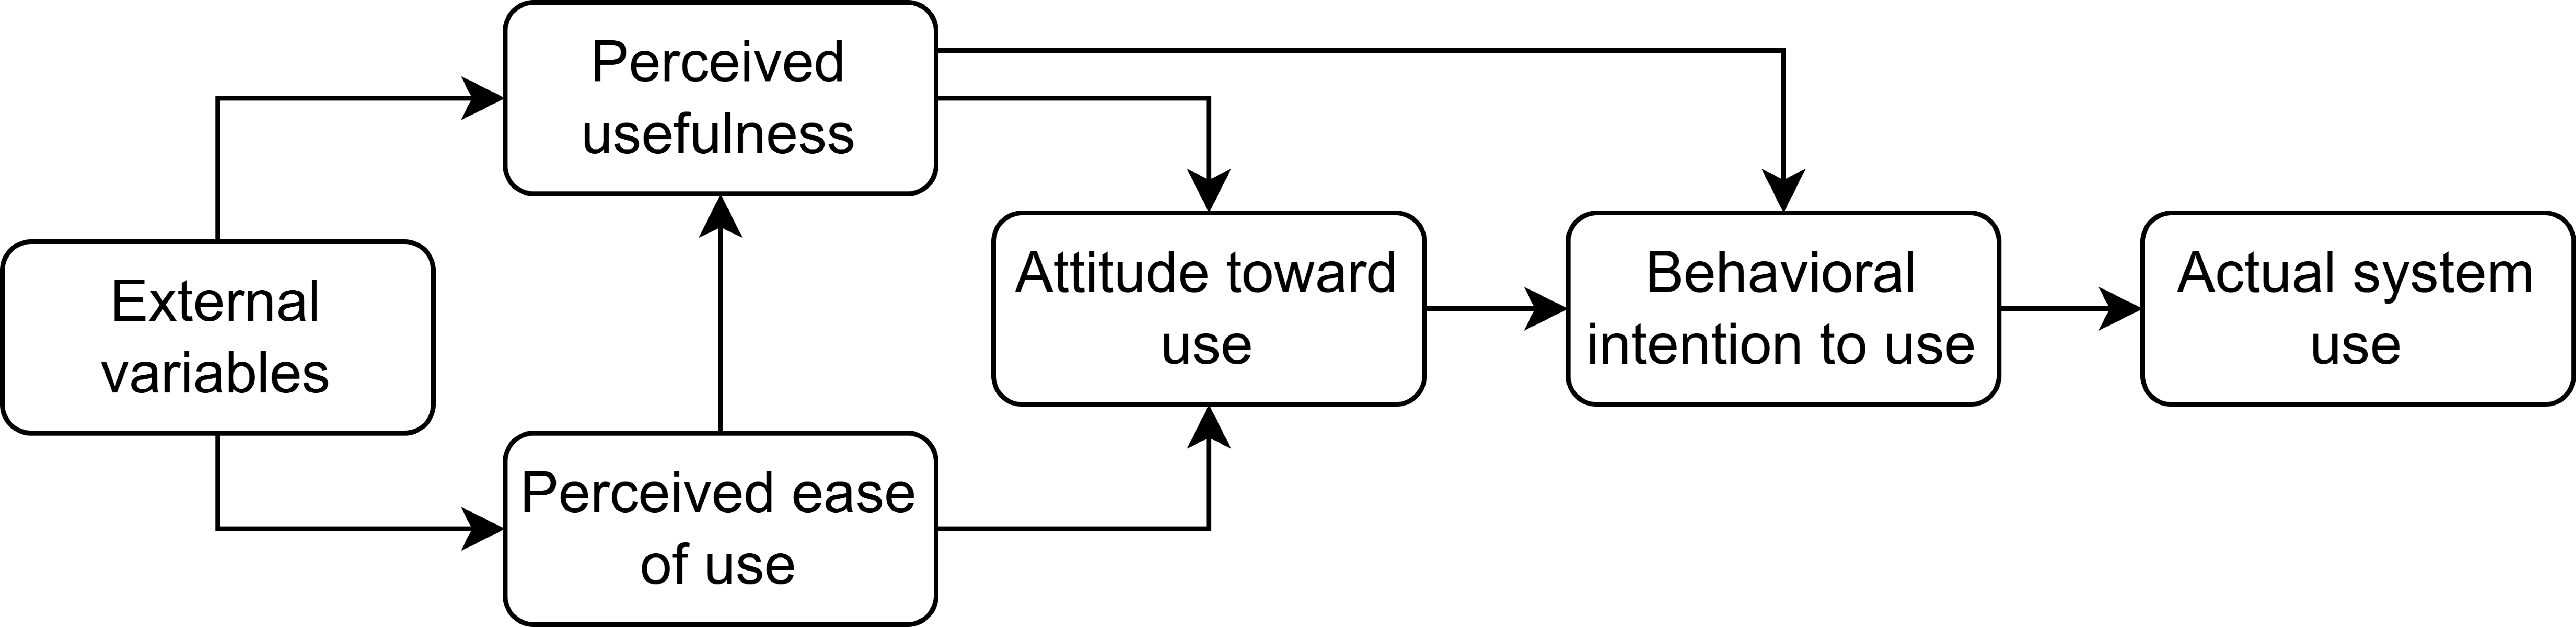
\includegraphics[width=2.5in]{img22}
        	\caption{Fases de evaluación del cuestionario TAM}
        	\label{fig:TAMEval}
        \end{figure}
        
        
        \subsubsection{Adaptación y aplicación}
        
        Para la aplicación y recolección de los datos del cuestionario se emplearon herramientas digitales que facilitaron el diseño, distribución y análisis de la información obtenida. La Tabla  \ref{tab:herramientas-analisis} presenta las principales herramientas utilizadas durante este proceso.
        
        \begin{table}[H]
        	\centering
        	\caption{Herramientas digitales utilizadas en la fase de diseño, recolección y análisis de datos de la encuesta}
        	\label{tab:herramientas-analisis}
        	\begin{tabular}{|c|p{5cm}|}
        		\hline
        		\textbf{Herramienta} & \textbf{Descripción} \\ \hline
        		Google Forms & Herramienta utilizada para la creación y aplicación del cuestionario de evaluación. \\ \hline
        		Excel & Utilizado para la organización de los datos y generación de gráficos. \\ \hline
        		R Studio & Empleado para el análisis estadístico de los datos recolectados. \\ \hline
        	\end{tabular}
        \end{table}
    
        \section{Metodología}
        El desarrollo de la aplicación móvil inclusiva se estructuró conforme a la \textit{Test-Driven Development Methodology for IoT Systems (TDDM4IoTS)}~\cite{GuerreroUlloa2020}, la cual consta de once fases orientadas a la trazabilidad, validación continua y control de calidad en sistemas humano–máquina. Este enfoque permitió mantener una correspondencia directa entre los requisitos del usuario, el diseño, la implementación y las pruebas del sistema. A continuación se detalla la aplicación práctica de cada fase, de modo que el proceso pueda ser replicado.
        
        \subsection{Roles del equipo}
        
        En esta sección se describen los roles utilizados para la ejecución del proyecto, así como las responsabilidades asumidas por cada uno durante el desarrollo y la evaluación de la aplicación móvil. La definición de estos roles permitió organizar las actividades del proyecto, facilitar la coordinación del equipo de trabajo y asegurar el cumplimiento de los entregables establecidos conforme a la metodología adoptada.

        \begin{table}[H]
        	\centering
        	\caption{Roles y encargos dentro del proyecto}
        	\begin{tabular}{|p{1cm}|p{\dimexpr\linewidth-2\tabcolsep-4cm}|}
        		\hline
        		\textbf{Rol} & \textbf{Encargo} \\ \hline
        		Project Facilitator &
        		Coordinó la ejecución del proyecto mediante la planificación de los entregables, la gestión de reuniones periódicas para el seguimiento de avances y la resolución de conflictos surgidos durante el desarrollo, con el fin de asegurar el cumplimiento de los objetivos establecidos. \\ \hline
        		
        		Counselor &
        		Actuó como experto técnico en áreas específicas del desarrollo, tales como inteligencia artificial, accesibilidad, seguridad y tecnologías de diseño web, brindando apoyo directo y asesoría técnica al equipo de desarrollo. \\ \hline
        		
        		Customer / End User &
        		Participó en las actividades de prueba y validación de requisitos, incluyendo usuarios con discapacidad visual y auditiva, así como usuarios sin discapacidad, con el objetivo de evaluar el funcionamiento, la accesibilidad y la adecuación de los requisitos de la aplicación móvil. \\ \hline
        		
        		Development Team &
        		Fue responsable de la ejecución de los entregables definidos, considerando la gestión del tiempo y los recursos disponibles para cada uno, así como la implementación de las funcionalidades del sistema conforme a los requerimientos establecidos. \\ \hline
        		
        	\end{tabular}
        \end{table}
        
        
        \subsection{Fase 1: Análisis preliminar}
        	
        En esta etapa se realizó el análisis de requisitos. Mediante una búsqueda bibliográfica se identificaron las principales funcionalidades accesibles de aplicaciones de mensajería actuales como WhatsApp, Messenger, Instagram y Telegram. Asimismo, se definieron criterios de accesibilidad, los cuales fueron evaluados mediante una lista de cotejo para 
        posteriormente verificar estudios similares que investigaron las limitaciones de las aplicaciones de mensajería.	    	
       
        Por otro lado, se llevó a cabo un análisis tecnológico, en el que se evaluaron distintas tecnologías que podrían aprovecharse en el desarrollo de la aplicación móvil. Posteriormente, se realizó un análisis de entorno y de viabilidad del sistema, con el fin de conocer tres aspectos principales: el público al que está orientado, las funciones que cumple y cómo ciertas tecnologías pueden ser aprovechadas para asegurar su despliegue y funcionamiento.  
        
       \subsubsection{Análisis de Requisitos}
        
        En esta etapa se realizarán dos tipos de análisis definidos por el cliente: los relacionados con el diseño de la aplicación móvil (requisitos no funcionales) y los referentes a la construcción de la parte lógica que permitirá el intercambio de mensajes (requisitos funcionales). Estos se organizarán por orden de prioridad para asegurar una implementación más rápida y efectiva.
        
        \subsubsection{Análisis de tecnología}
        
        En esta etapa se identificaron los recursos tecnológicos que apoyen a satisfacer los requisitos del sistema mediante un estudio de viabilidad técnica y económica, comparando frameworks móviles (Flutter, React Native y Kotlin), bases de datos (PostgreSQL, MySQL) y APIs de IA (Google Cloud Speech, IBM Watson, Whisper). React Native y PostgreSQL fueron seleccionadas por su portabilidad y desempeño, mientras que se elegieron modelos de IA como Whisper debido a que son libres y precissas teniendo una alta disponibilidad en entornos offline, tambien se evaluo el hardware disponible, así como las herramientas necesarias para la configuración y el despliegue.
        
        \subsubsection{Análisis del entorno}
        
       	En esta etapa se evaluó la viabilidad de implementación del sistema considerando el entorno de uso y el entorno técnico de ejecución. Se identificó que el aplicativo debía ofrecer funcionalidades de conversión de mensajes de texto a audio y de audio a texto, con el objetivo de facilitar la comunicación de usuarios con discapacidades visuales y auditivas.
       	
       	Además, se analizó el entorno técnico necesario para garantizar un procesamiento estable y eficiente de los mensajes. Para ello, se investigaron y compararon distintas APIs de inteligencia artificial mediante el análisis de su documentación oficial y pruebas preliminares, seleccionando aquellas que aseguraban un desempeño confiable y que fueran ofline. Finalmente, se configuraron dos servidores web con el propósito de distribuir la carga de trabajo, mejorar la disponibilidad del sistema y garantizar su estabilidad durante el uso concurrente de la aplicación.
       	
       	\subsection{Fase 2: Diseño de la capa tecnológica}
       	
       	En esta fase se desarrolló un diseño inicial de la aplicación móvil, el cual sirvió como base para la construcción del sistema. Se definió la arquitectura completa del sistema, así como la planificación y configuración del entorno de trabajo, apoyándose en herramientas de modelado como PowerDesigner, que permitieron un diseño estructurado del desarrollo. El uso de estas herramientas facilitó el proceso al brindar soporte para la creación de una arquitectura más robusta, reduciendo errores y acelerando la generación de diagramas.
       	
       	Como resultado de este proceso de análisis y diseño, y con base en los requerimientos previamente definidos, se estableció una arquitectura de tres capas: (i) presentación, (ii) lógica de negocio y (iii) persistencia de datos. La capa de presentación se desarrolló en React Native, garantizando compatibilidad con Android 10 o superior. La capa lógica, implementada en Spring Boot 3 (Java) y Python 3.10, integra módulos de reconocimiento de voz, síntesis de voz y corrección de comandos mediante inteligencia artificial. La capa de datos utiliza PostgreSQL 13, incorporándose además RabbitMQ para la mensajería asincrónica y Docker Compose para el despliegue modular. La selección de estas tecnologías se sustentó en un análisis comparativo de rendimiento y consumo energético, priorizando componentes de ejecución local frente a dependencias en la nube, conforme a los lineamientos de TDDM4IoTS para IoT distribuido.
       	
       	\subsection{Fase 3: Análisis detallado de requisitos}
       	
       	En esta fase, para cada funcionalidad del sistema, se detallaron los requisitos correspondientes. Se utilizaron herramientas compatibles con el lenguaje UML (Lenguaje de Modelado Unificado), como PowerDesigner, para asegurar que cada funcionalidad fuera comprendida claramente. Se emplearon diagramas de casos de uso mediante sus respectivas plantillas, lo cual facilitó la comprensión de las funcionalidades y ayudó a eliminar cualquier posible confusión.
       	
       	
       	
       	
       	\subsection{Fase 4: Generación y adaptación de modelos}
       	
       	En esta etapa, el objetivo principal fue aumentar la productividad en el desarrollo, aprovechando los modelos creados en las fases anteriores de la metodología. Estos modelos permitieron generar representaciones más específicas que facilitaron la comprensión del problema. Es decir, a partir de una idea abstracta o general del diagrama, se utilizaron herramientas que permitieron crear diagramas detallados. Por ejemplo, herramientas como PowerDesigner permitieron generar directamente un diagrama de base de datos a partir de un diagrama de clases, lo que agilizó las tareas relacionadas con la arquitectura del software.
       	
       	\subsection{Fase 5: Generación de pruebas}
       	
       	En el desarrollo de software, las pruebas fueron un componente clave, ya que garantizaron que los requisitos del sistema se cumplieran, asegurando un producto de calidad. Las pruebas se dividieron en dos grupos:
       	
       	\begin{itemize}
       		\item \textbf{Escritas por desarrolladores}: En esta etapa, se escribieron pruebas para la API de inteligencia artificial para obtener tiempos de respuestas en el procesamiento de los recursos.  Asimismo mediante una aplicación de Google se evaluo la accesibilidad de la aplicación, mejorando las advertencia que nos ofrecia y asegurando la calidad del software.  
       		
       		\item \textbf{Escritas por clientes}: En esta fase, cada funcionalidad del sistema fue validada por el equipo de desarrollo y posteriomente por el Project facilitator, quien verificó si el sistema cumplía con los requisitos y expectativas esperadas. Asimismo, se realizaron pruebas con 25 usuarios reales mediante el cuestionario TAM para evaluar la Utilidad percibida y Facilidad de uso percibida y con ello verificar si la aplicación era aceptada por los usuarios evaluados.
       	\end{itemize}
       	
	     \subsection{Fase 6: Generación de software}
	     
	     En esta fase del desarrollo, se validó que el código generado fuera correcto. Se procedió a verificar, corregir o agregar la lógica de negocios que no se hubiera implementado adecuadamente. Para la creación de las API se utilizó el framework de servicios web Java Spring Boot, y los servicios desarrollados fueron consumidos por la aplicación móvil, desarrollada en React Native, aprovechando las ventajas multiplataforma de este framework. Una vez finalizada la generación del software, se realizó una revisión para asegurar el correcto funcionamiento del sistema. Asimismo, con los modelos definidos en la etapa cuatro de la metodología se obtuvo la API de mensajería, y el uso del framework tanto en el backend como en el frontend permitió crear interfaces y modelos de manera más rápida, agilizando el desarrollo. 
	  
         \subsection{Fase 7: Refinamiento de modelos}
         
         En esta etapa, el objetivo fue obtener un modelo más estructurado en comparación con la versión inicial. Para ello, se realizaron ajustes que mejoraron la escalabilidad y robustez de los modelos, asegurando la calidad en la construcción de la aplicación. La arquitectura inicial de la aplicación móvil se analizó para optimizar el envío y la recepción de mensajes, lo que mejoró considerablemente la estabilidad en la transmisión de los mismos.
         
        \subsection{Fase 8: Refinamiento de software}
        
        En esta etapa se garantizó la calidad del software mediante la eliminación de redundancias en el código y la refactorización para mejorar su legibilidad y facilitar el mantenimiento del sistema. Esto implicó seguir buenas prácticas de programación. Para llevar a cabo estas tareas, se utilizarán los procesos y herramientas que el IDE elegido proporciona a los desarrolladores.
        
        \subsection{Fase 9: Implementación de hardware y software}
        
        En esta etapa se llevó a cabo la configuración de los componentes de hardware y software según lo especificado en el proyecto, con el objetivo de poner en funcionamiento el software desarrollado. Esto garantizó que los requerimientos finales establecidos entre el cliente y el desarrollador se cumplieran. En caso de que el proyecto sufriera cambios posteriores, se ajustó la infraestructura para integrar las modificaciones y verificar que todo funcionara correctamente con la nueva actualización, asegurando una integración segura al sistema.
        
        Para ello el sistema se desplegó en un entorno híbrido: servidor CentOS 7 (backend, PostgreSQL) y servicios AWS EC2 (GPU NVIDIA) para los modelos de IA. La aplicación móvil fue compilada en formato APK y distribuida para pruebas de campo en dispositivos Android 10 +.  
        
        Se documentó el proceso de instalación, configuración de contenedores y credenciales de acceso para reproducibilidad.
        
        \subsection{Fase 10: Evaluación de entregables}
        
        En esta sección se evaluaron los entregables del proyecto, incluyendo la aplicación móvil y la documentación. Se utilizó un cronograma que especifica entregables, componentes y tareas, asegurando que todas las actividades se completaron según lo planificado.
        
        \subsection{Fase 11: Mantenimiento}
        
        Esta etapa se centró en implementar mejoras, ajustes y correcciones necesarias en la aplicación o su infraestructura. En el caso del proyecto, esta etapa no se ha aplicado, ya que el sistema cumple con los requisitos establecidos; sin embargo, se incluyen sugerencias de mantenimiento que podrían implementarse en el futuro para garantizar la estabilidad y funcionamiento óptimo del sistema a largo plazo.
        
       	\subsection{-----}
        
        \subsection{Fase 1: System Requirements Definition (SRD)}
        Durante esta fase se identificaron las necesidades del proyecto mediante un proceso combinado de revisión sistemática de literatura, entrevistas y encuestas iniciales.  
        La revisión sistemática se realizó siguiendo la guía PRISMA y el protocolo de Kitchenham, abarcando los años 2018–2025 en bases de datos IEEE Xplore, ACM DL, Scopus y ScienceDirect. Los criterios de inclusión consideraron estudios sobre aplicaciones accesibles, mensajería inclusiva, y tecnologías de conversión voz–texto o texto–voz. 
         
        El análisis de 62 artículos permitió identificar 14 funcionalidades recurrentes, de las cuales 9 se consideraron viables para integrar en la aplicación.  
        Posteriormente, se efectuaron entrevistas semiestructuradas con 10 usuarios con discapacidades visuales, auditivas y del habla, además de tres especialistas en accesibilidad digital. Los resultados se complementaron con una encuesta a 45 participantes, que reveló como principales requerimientos la comunicación multimodal, la simplicidad de interfaz y la seguridad de los mensajes.  
        
        Finalmente, se efectuó un estudio de viabilidad técnica y económica, comparando frameworks móviles (Flutter, React Native y Kotlin), bases de datos (PostgreSQL, MySQL) y APIs de IA (Google Cloud Speech, IBM Watson, Whisper). React Native y PostgreSQL fueron seleccionadas por su portabilidad y desempeño, mientras que Whisper se eligió por su precisión en entornos offline.
        
        \subsection{Fase 2: System Architecture Design (SAD)}
        Con base en los requerimientos definidos, se diseñó una arquitectura de tres capas: (i) presentación, (ii) lógica de negocio, y (iii) persistencia de datos.  
        La capa de presentación se desarrolló en React Native 0.74, garantizando compatibilidad con Android 10 +.  
        La capa lógica, implementada en Spring Boot 3 (Java) y Python 3.10, integra módulos de reconocimiento de voz, síntesis de voz y cifrado.  
        La capa de datos utiliza PostgreSQL 13. Se incorporó RabbitMQ para la mensajería asincrónica y Docker Compose para el despliegue modular.  
        La selección de tecnologías se sustentó en un análisis comparativo de rendimiento y consumo energético, priorizando componentes de ejecución local frente a dependencias en la nube, conforme a los lineamientos de TDDM4IoTS para IoT distribuido.
        
        \subsection{Fase 3: Module Requirements Definition (MRD)}
        Se definieron los requisitos funcionales y métricas específicas para cada módulo:  
        \begin{itemize}
            \item \textbf{Speech Processing Module}: precisión mínima del 95 \% en transcripción, latencia < 300 ms.  
            \item \textbf{Text-to-Speech Module}: inteligibilidad $\geq$ 4.5/5 según escala MOS.  
            \item \textbf{Image Understanding Module}: descripción correcta en $\geq$ 90 \% de las pruebas con dataset BLIP. 
            \item \textbf{Accessibility Interface Module}: navegación por voz completa y compatibilidad con lectores de pantalla.  
            \item \textbf{Encryption Module}: cifrado AES-256 con clave RSA de intercambio.  
        \end{itemize}
        Cada requisito fue validado con los expertos del proyecto para asegurar alineación con las necesidades de accesibilidad identificadas en la fase SRD.
        
        \subsection{Fase 4: Module Architecture Design (MAD)}
        En esta fase se elaboraron diagramas UML de clases y secuencia, definiendo las interfaces entre módulos y las API de comunicación.  
        Los datos se transfieren en formato JSON mediante WebSocket, permitiendo baja latencia en la mensajería en tiempo real.  
        El módulo de accesibilidad gestiona la configuración del usuario para adaptar el modo de interacción (voz, texto o imagen), en concordancia con los principios de diseño inclusivo.
        
        \subsection{Fase 5: Module Test Design (MTD)}
        Se diseñaron pruebas unitarias y funcionales antes de la implementación (\textit{test-first}).  
        Cada módulo incluye al menos 25 casos de prueba automatizados en \texttt{JUnit} 5 y \texttt{pytest}.  
        Se definieron criterios de aceptación cuantitativos: exactitud $\geq$ 95 \%, tiempo medio de respuesta < 400 ms y consumo de CPU < 30 \%.  
        El conjunto de datos de validación incluyó audios del corpus Mozilla Common Voice (español) y descripciones visuales del dataset VizWiz.
        
        \subsection{Fase 6: Module Implementation (MI)}
        La codificación se realizó siguiendo los principios SOLID y control de versiones en GitLab.  
        El equipo de desarrollo estuvo conformado por: un líder técnico, dos desarrolladores (full-stack y IA), un diseñador UX/UI con especialidad en accesibilidad y un responsable de pruebas.  
        Se emplearon VS Code, Android Studio Hedgehog y Jupyter Lab como entornos de trabajo.  
        Los modelos de IA (Whisper ASR y pyttsx3 TTS) fueron integrados en contenedores Docker para asegurar reproducibilidad y portabilidad.
        
        \subsection{Fase 7: Module Testing (MT)}
        Se ejecutaron las pruebas unitarias y funcionales definidas.  
        Los módulos alcanzaron un promedio de 93.8 \% de cobertura y 98.1 \% de éxito en las pruebas.  
        El control de calidad se automatizó mediante pipelines CI/CD en GitLab, que validan cada \textit{commit} antes de la integración.
        
        \subsection{Fase 8: System Integration (SI)}
        La integración se realizó de manera incremental, validando la interoperabilidad entre los módulos a través de RabbitMQ y REST APIs.  
        Se desarrollaron pruebas de sincronización y tolerancia a fallos, simulando redes 4G y Wi-Fi inestables.  
        El sistema mostró una resiliencia superior al 96 \% en la entrega de mensajes tras interrupciones breves.
        
        \subsection{Fase 10: System Deployment (SD)}
        El sistema se desplegó en un entorno híbrido: servidor CentOS 7 (backend, PostgreSQL) y servicios AWS EC2 (GPU NVIDIA) para los modelos de IA. La aplicación móvil fue compilada en formato APK y distribuida para pruebas de campo en dispositivos Android 10 +.  
        
        Se documentó el proceso de instalación, configuración de contenedores y credenciales de acceso para reproducibilidad.
        
        \subsection{Fase 10: Evaluación de los entregables}
        El sistema completo fue evaluado mediante pruebas de usabilidad, accesibilidad y rendimiento.  Se aplicó el modelo \textit{Technology Acceptance Model (TAM)} con 40 usuarios: 16 con discapacidad visual, 14 auditiva y 10 del habla.
        
        El cuestionario TAM incluyó 24 ítems distribuidos en cuatro constructos: utilidad percibida, facilidad de uso, actitud hacia el uso e intención de adopción.  Cada ítem se midió en escala Likert de 1 a 5.
        
        Los datos se analizaron con SPSS v29, obteniéndose un coeficiente $\alpha$ de Cronbach = 0.92 y una media de aceptación de 4.61. Las pruebas funcionales alcanzaron una precisión global del 97.3 \% en transcripción y una latencia promedio de 312 ms.
            
        \subsection{Fase 11: System Maintenance and Evolution (SME)}
        Finalmente, se estableció un plan de mantenimiento correctivo y evolutivo.  Las métricas de desempeño recolectadas se almacenan en un panel Grafana conectado a Prometheus.
          
        Las actualizaciones incluyen la incorporación de OCR para lectura de documentos, nuevos idiomas de voz y soporte para mensajería grupal.  
        Asimismo, se definió una política de versiones semestrales (\textit{rolling release}) y un protocolo de retroalimentación continua con los usuarios.
        
        \bigskip
        La aplicación rigurosa de las once fases de TDDM4IoTS permitió una trazabilidad completa desde la definición de requerimientos hasta la validación final, garantizando reproducibilidad, calidad del software y accesibilidad inclusiva dentro del marco de los sistemas humano–máquina.
        
    

\section{Resultados}

\noindent Los resultados que se obtuvieron a aplicar la metodologia Tddt4iots basada en este desarrollo de software se muestran a continuación.

\subsection {Análisis preliminar}

\noindent Para la implementación del sistema se tomaron en cuenta aspectos de análisis de requisitos, tecnología, entorno y viabilidad, permitiendo tener un desarrollo integro y bien estructurado para las fases próximas de la metodologia. Debido a que se tiene en cuenta las necesidades reales de desarrollo, implementación y prueba del sistema.

\subsubsection {Análisis de requisitos}

\noindent En esta subfase análisis de requisitos se realizó una revisión bibliográfica que permitió identificar estudios con la línea investigativa de este proyecto. Con ello se analizaron sistemas similares, sus funcionalidades, tecnologías aplicadas y limitantes, lo ayudó a estructurar de manera más sólida los requisitos del software.

\begin{itemize}
	
	\item \textbf{Accesibilidad en aplicaciones de mensajería utilizadas:} En la Tabla \ref{tab:caracteristicas-mensajeria} se muestran las características inclusivas que presentan algunas de las aplicaciones de mensajería. 
	
	
	\begin{table}[h!]
		\centering
		\caption{Características inclusivas en aplicaciones de mensajería actuales}
		\label{tab:caracteristicas-mensajeria}
		\begin{tabular}{|p{1.5cm}|p{1.5cm}|p{1.5cm}|p{1.5cm}|}
			\hline
			\textbf{WhatsApp} & \textbf{Telegram} & \textbf{Messenger} & \textbf{Instagram} \\
			\hline
			La aplicación es compatible con lectores de pantalla como TalkBack y VoiceOver. & Compatibilidad con TalkBack y VoiceOver. & Compatibilidad con lectores de pantalla. & Compatibilidad con lector de pantalla. \\
			\hline
			Ajustar pantalla o tamaño de la fuente. & Ajuste de volumen en los chats de voz de forma individual por cada usuario. & Ajuste de contraste de la aplicación. & Administración de subtítulos en videos o teclas. \\
			\hline
			Agrandar la imagen de manera temporal. & Las fotos y videos pueden expandirse directamente desde el chat. & Cambio de colores de los chats. & El texto alternativo describe imágenes para usuarios con lector de pantalla. \\
			\hline
			Ajustar contraste de los colores. & & Cambio de color del estado activo. & El tamaño del texto puede ajustarse desde la configuración del dispositivo o del navegador. \\
			\hline
			Transcripciones de audio a texto & & & \\
			\hline
		\end{tabular}
	\end{table}
	
	
	\item \textbf{Lista de cotejo:} En la Tabla 6 se muestra una lista de cotejo que describe los criterios obtenidos de los recursos investigados \cite{Swati2021,w3c2008,Ballantyne2018,AcostaVargas2020}.
	
	\begin{multicols}{2}
		\begin{enumerate}
			\item Distinción de elementos habilitados y deshabilitados
			\item Transcripción de vídeos
			\item Transcripción de audio
			\item Transcripción de audio en tiempo real
			\item Identificador de contenido alternativo
			\item Tamaño de texto
			\item Fuentes de texto
			\item Color de texto y contraste
			\item Contraste
			\item Velocidad de voz sintetizada
			\item Volumen de voz
			\item Volumen global
			\item Sugerencias de error
			\item Lenguaje de señas
		\end{enumerate}
	\end{multicols}
	
	\begin{table}[ht]
		\centering
		\caption{Lista de costo de aplicaciones de mensajería}
		\label{tab:costo-aplicaciones}
		\begin{tabular}{|c|c|c|c|c|}
			\hline
			\textbf{No.} & \textbf{WhatsApp} & \textbf{Telegram} & \textbf{Messenger} & \textbf{Instagram} \\
			\hline
			1 & X & X & X & X \\
			\hline
			2 & X & X & X & $\checkmark$ \\
			\hline
			3 & $\checkmark$ & X & X & X \\
			\hline
			4 & X & X & X & X \\
			\hline
			5 & X & X & X & X \\
			\hline
			6 & $\checkmark$ & $\checkmark$ & X & X \\
			\hline
			7 & X & X & X & X \\
			\hline
			8 & X & X & X & X \\
			\hline
			9 & $\checkmark$ & $\checkmark$ & $\checkmark$ & $\checkmark$ \\
			\hline
			10 & $\checkmark$ & X & X & X \\
			\hline
			11 & X & X & X & X \\
			\hline
			12 & $\checkmark$ & $\checkmark$ & $\checkmark$ & $\checkmark$ \\
			\hline
			13 & $\checkmark$ & $\checkmark$ & $\checkmark$ & $\checkmark$ \\
			\hline
			14 & X & X & X & X \\
			\hline
		\end{tabular}
	\end{table}
	
	
		\item \textbf{Evaluación de aplicaciones basada en estudios previos:} A continuación, se recopilan los aspectos limitantes de las aplicaciones.
	
		\begin{itemize}
			\item \textbf{WhatsApp}
			\begin{enumerate}
				\item Dificultades para operar la interfaz por falta de encabezados, etiquetas o textos alternativos que dificultan la identificación.
				\item Dificultad para percibir la ubicación dentro del sistema.
				\item Dificultad para percibir submenús.
				\item Retroalimentación sonora dentro de la aplicación \cite{Ferreira2016,Huang2025}.
			\end{enumerate}
			
			\item \textbf{Messenger}
			\begin{enumerate}
				\item El resaltado de los íconos del menú inferior presenta un contraste demasiado bajo.
				\item Ciertas opciones que se despliegan al mantener presionado un botón aumentan la complejidad de las tareas \cite{Ferreira2016,Huang2025}.
			\end{enumerate}
			
			\item \textbf{Instagram}
			\begin{enumerate}
				\item El ícono de envío de mensajes directos, ubicado en la esquina superior derecha, es idéntico al ícono de compartir publicaciones.
				\item Los íconos del perfil que representan “Tus publicaciones”, “Fotos” y “Videos” tienen un bajo resaltado, dificultando su visualización.
				\item Los íconos de “burbujas” en la página inicial pueden interpretarse como botones para crear publicaciones o enviar mensajes directos.
				\item Las etiquetas de “video” y “foto” en la creación de publicaciones se interpretan como botones.
				\item La ubicación de la página de perfil no es clara.
				\item No es claro si el ícono de compartir está debajo de una publicación.
				\item Las publicaciones del \textit{feed} no parecen desplazables debido al mal contraste entre el menú inferior y el fondo blanco, lo que puede generar confusión \cite{Ferreira2016,Huang2025}.
				\item Existen dos funciones para agregar contenido: una para historias (parte superior izquierda) y otra con el signo de adjunto (menú inferior).
				\item Doble funcionalidad para compartir: en los tres puntos de la publicación y con el ícono del avión debajo de la misma.
				\item Las sugerencias de contactos pueden interrumpir la página principal del \textit{feed}.
			\end{enumerate}
			
			\item \textbf{Telegram}
			
			Algunos usuarios han expresado quejas en las reseñas de Google Play, evidenciando problemas de usabilidad y accesibilidad. Se menciona la necesidad de mejorar aspectos como el contraste de colores, la ayuda ante errores y la consistencia en íconos y submenús. Estas limitaciones pueden afectar la experiencia de ciertos usuarios y la accesibilidad general de la aplicación \cite{Rumini2019}.
		\end{itemize}
	
		\item \textbf{Limitaciones de aplicaciones} En la Tabla \ref{tab:limitaciones-aplicaciones} se menciona el problema identificado generalmente en las aplicaciones móviles con su respectiva descripción \cite{Huang2025,CaroAlvaro2018,Griggio2024}. 
		
		\begin{table}[ht]
			\centering
			\caption{Limitaciones de aplicaciones}
			\label{tab:limitaciones-aplicaciones}
			\begin{tabular}{|p{2cm}|p{6cm}|}
				\hline
				\textbf{Problema} & \textbf{Descripción} \\
				\hline
				Textos de la aplicación demasiados pequeños & El uso de mensajes de entrada o ventanas emergentes es difícil de leer. \\
				\hline
				Uso indiscriminado de ventanas emergentes & Las ventanas emergentes o notificaciones pueden dificultar el uso normal de la aplicación. \\
				\hline
				Textos recortados & Los textos recortados pueden dificultar la visualización de los textos de un menú o aviso. \\
				\hline
				Falta de textos alternativos en medios visuales & Los lectores de pantalla leen el texto alternativo de las imágenes, pero a veces este no está configurado o es inaccesible. \\
				\hline
				Interpretación de mensajes con emojis & Los lectores de pantalla interpretan mal los mensajes con emojis, sobre todo cuando se combinan varios. \\
				\hline
				Iconos engañosos & En las aplicaciones de mensajería, algunos íconos pueden tener funciones distintas a las esperadas, lo que confunde al usuario. \\
				\hline
				Interfaz de usuario poco clara & En la interfaz es difícil saber en qué submenu se está posicionado y, además, dónde se puede encontrar una determinada opción. \\
				\hline
				Latencia del sistema & El sistema puede presentar tavas al cargar un submenu u opción. \\
				\hline
				Enfoques similares con resultados diferentes & Algunas opciones de las aplicaciones pueden parecer iguales, pero al usarlas ofrecen resultados distintos, lo que causa confusión al usuario. \\
				\hline
				Opciones excesivas y Desorden visual & La aplicación puede incluir demasiadas opciones en una pestaña, desordenadas o mal agrupadas, lo que confunde al usuario. \\
				\hline
			\end{tabular}
		\end{table}
		
		
		\item \textbf{Análisis: funciones de accesibilidad y limitaciones en WhatsApp, Messenger, Telegram e Instagram} Se observo que muchas aplicaciones de mensajería como WhatsApp, Messenger, Telegram e Instagram ya incorporan funciones de accesibilidad. Sin embargo, aún presentan limitaciones \cite{Zahida2021,Swati2021,Rumini2019}. Estas aplicaciones ofrecen características comunes, como compatibilidad con lectores de pantalla y opciones de ajuste texto o contraste.
		Algunas han avanzado más en este aspecto. Por ejemplo, WhatsApp ha añadido la transcripción de audios en sus últimas actualizaciones, lo que muestra un progreso constante en estas funciones accesibles \cite{Meta2025}. Instagram ha implementado subtítulos en sus videos \cite{Meta2025}, mientras que plataformas como Facebook Messenger aún no cuentan con esta opción. Telegram, al ser más abierta al público, ha mejorado en accesibilidad \cite{telegram2025}, aunque sigue en desventaja frente a WhatsApp, Messenger e Instagram.
		A pesar de estas diferencias, es posible identificar un conjunto de funciones accesibles que se repiten en las aplicaciones de mensajería y que resultan de gran apoyo para personas con discapacidades visuales o auditivas. A continuación, se presenta una lista de estas características:
		

		\begin{itemize}
			\item Compatibilidad con lectores de pantalla (TalkBack y VoiceOver).
			\item Ajuste de contraste para mejorar la visibilidad del contenido.
			\item Elementos visibles por lector de pantalla, lo que permite interpretar textos e imágenes.
			\item Tamaño del objetivo táctil ajustado para facilitar la interacción con botones y controles.
			\item Sugerencias de error automáticas en caso de fallos al ingresar datos.
			\item Idioma de la aplicación identificado correctamente para lectores de pantalla.
		\end{itemize}
		
		\item \textbf{Colores de aplicación} 
		\noindent Para definir los colores de la aplicación, WCAG establece pautas que ayudan a verificar si el color usado es adecuado para la accesibilidad en una aplicación móvil. Estas pautas \cite{WCAG22} se organizan en tres niveles: A, AA y AAA. El nivel A indica que no se debe usar únicamente el color para transmitir información, ya que no todas las personas perciben los colores de la misma manera. Por eso, se recomienda incluir otros métodos, como solicitar una respuesta o diferenciar un elemento visual, de modo que todos los usuarios puedan acceder a la información sin importar sus capacidades visuales.
		
		\noindent Por otro lado, el nivel AA establece como objetivo que el texto sea legible para más personas. Para lograrlo, se requiere un contraste suficiente entre el fondo y el texto, ya que algunas personas no pueden leer textos con bajo nivel de visibilidad. De esta manera, se indica que los textos grandes y las imágenes de texto de gran tamaño deben tener una relación de contraste mínima de 3:1, mientras que los textos normales deben alcanzar al menos 4,5:1.
		 
		\noindent El nivel AAA establece que el texto debe ser accesible también para personas que necesitan un contraste más fuerte con respecto al fondo, ya que algunas no pueden leer textos con un contraste mínimo. Por ello, este nivel indica que los textos grandes y las imágenes de texto de gran tamaño deben tener una relación de contraste de al menos 4,5:1, mientras que los textos normales deben alcanzar al menos 7:1. En este sentido, WCAG define fórmulas para calcular el contraste y compararlo con los valores establecidos, lo que permite determinar si es adecuado aplicar un color específico.
		
		\noindent Así, se indica que el texto en negrita se considera más grande, lo que facilita su lectura debido al contraste, mientras que un texto fino puede resultar más difícil de distinguir \cite{WCAG22}.
		
		\noindent En la Fig. \ref{fig:normalizacion-rgb} se presenta la primera fórmula, la cual permite normalizar el color RGB que se usará en las fórmulas posteriores. 
		
		\begin{figure}[ht]
			\centering
			\caption{Normalización de color RGB}
			\label{fig:normalizacion-rgb}
			\[
			\begin{aligned}
				R_{sRGB} &= \frac{R_{8bit}}{255} \\
				G_{sRGB} &= \frac{G_{8bit}}{255} \\
				B_{sRGB} &= \frac{B_{8bit}}{255}
			\end{aligned}
			\]
			\small\textbf{FUENTE: WCAC \cite{W3CLuminance2021}}
		\end{figure}
	
		\noindent En la Fig. \ref{fig:calculo-luminancia} se muestra la fórmula de cálculo de luminancia, que permite obtener los valores (L) necesarios para la fórmula de contraste. Es importante normalizar correctamente los valores y aplicar de manera adecuada las condicionales y constantes. RSRGB, GSRGB y BSRGB corresponden al color RGB normalizado.
		
		\begin{figure}[ht]
			\centering
			\caption{Cálculo de la luminancia}
			\label{fig:calculo-luminancia}
			\footnotesize % Fuente aún más pequeña
			\setlength{\abovedisplayskip}{2pt} % Reduce espacio antes de ecuación
			\setlength{\belowdisplayskip}{2pt} % Reduce espacio después de ecuación
			\[
			\begin{aligned}
				&\text{If } R_{sRGB} \leq 0.03928 \text{ then} \\
				&\qquad R = \frac{R_{sRGB}}{12.92} \\
				&\text{otherwise} \\
				&\qquad R = \left( \frac{R_{sRGB} + 0.055}{1.055} \right)^{2.4} \\
				&\text{If } G_{sRGB} \leq 0.03928 \text{ then} \\
				&\qquad G = \frac{G_{sRGB}}{12.92} \\
				&\text{otherwise} \\
				&\qquad G = \left( \frac{G_{sRGB} + 0.055}{1.055} \right)^{2.4} \\
				&\text{If } B_{sRGB} \leq 0.03928 \text{ then} \\
				&\qquad B = \frac{B_{sRGB}}{12.92} \\
				&\text{otherwise} \\
				&\qquad B = \left( \frac{B_{sRGB} + 0.055}{1.055} \right)^{2.4}
			\end{aligned}
			\]
			\vspace{0.1cm}
			\scriptsize\textbf{FUENTE: WCAG \cite{W3CLuminance2021}} % Fuente muy pequeña
		\end{figure}
		
		\noindent En la \ref{fig:formula-luminancia} se presenta la fórmula de luminancia, la cual se aplica después de normalizar y condicionar los valores RGB.
		
		\begin{figure}[ht]
			\centering
			\caption{Fórmula de luminancia}
			\label{fig:formula-luminancia}
			\begin{equation*}
				L = 0.2126 \cdot R + 0.7152 \cdot G + 0.0722 \cdot B
			\end{equation*}
			\small\textbf{FUENTE: WCAG \cite{W3CLuminance2021}}
		\end{figure}
		
		\noindent En la Fig. \ref{fig:formula-contraste} se muestra la fórmula de contraste, la cual genera valores en un rango de 1:1 a 21:1 \cite{W3CContrast2012}. En esta fórmula, L1 corresponde a la luminancia relativa del color más claro y L2 a la del color más oscuro. El valor 0.05 se incluye para evitar la división por cero.
		
		\begin{figure}[ht]
			\centering
			\caption{Fórmula de contraste}
			\label{fig:formula-contraste}
			\[
			\text{contrast\_ratio} = \frac{L_2 + 0.05}{L_1 + 0.05}
			\]
			\vspace{0.2cm}
			\small\textbf{FUENTE: WCAG \cite{W3CContrast2012}}
		\end{figure}
		
		\noindent Ejemplo aplicando las fórmulas: Supongamos que tenemos la siguiente matriz con dos colores RGB:
		
		\begin{table}[ht]
			\centering
			\caption{Matriz inicial RGB}
			\label{tab:matriz-inicial-rgb}
			\begin{tabular}{|c|c|c|c|c|}
				\hline
				& \textbf{R} & \textbf{G} & \textbf{B} & \textbf{Color} \\
				\hline
				Color L1 (RGB) & 37 & 142 & 245 & \\
				\hline
				Color L2 (RGB) & 97 & 102 & 97 & \\
				\hline
			\end{tabular}
		\end{table}
		
		\noindent Aplicando la fórmula de la Fig. \ref{fig:normalizacion-rgb} normalizamos los valores de la matriz:
		
		\begin{table}[ht]
			\centering
			\caption{Normalización de valores RGB}
			\label{tab:normalizacion-rgb}
			\begin{tabular}{|c|c|c|c|}
				\hline
				\textbf{F} & \textbf{RSRGB} & \textbf{GsRGB} & \textbf{BsRGB} \\
				\hline
				Normalizar (L1) & 0,145098039 & 0,556862745 & 0,960784314 \\
				\hline
				Normalizar (L2) & 0,380392157 & 0,4 & 0,380392157 \\
				\hline
			\end{tabular}
		\end{table}
							
		\noindent Posteriormente, aplicando las condiciones y fórmulas de la Fig. \ref{fig:calculo-luminancia}, se obtiene la siguiente matriz. condicionamos:

			
		\begin{table}[H]
			\centering
			\caption{Condiciones de valores RGB}
			\label{tab:condiciones-rgb}
			\begin{tabular}{|c|c|c|c|}
				\hline
				& \textbf{RsRGB $\leq$ 0,03928} & \textbf{GsRGB $\leq$ 0,03928} & \textbf{BsRGB $\leq$ 0,03928} \\
				\hline
				\textbf{L1} & FALSO & FALSO & FALSO \\
				\hline
				\textbf{L2} & FALSO & FALSO & FALSO \\
				\hline
			\end{tabular}
		\end{table}
		
				
		\noindent Se calcula de la siguiente manera: si la condicion es verdadera, se aplica la primera parte de la fórmula de la Fig. \ref{fig:calculo-luminancia} $R = \frac{R_{sRGB}}{12.92}$, en caso contrario $R = \left( \frac{R_{sRGB} + 0.055}{1.055} \right)^{2.4}$;  obteniéndose como resultado la siguiente matriz:
		
		\begin{table}[H]
			\centering
			\caption{Valores resultantes de L1 y L2}
			\label{tab:valores-resultantes-L1-L2}
			\begin{tabular}{|c|c|c|c|}
				\hline
				& \textbf{R} & \textbf{G} & \textbf{B} \\
				\hline
				\textbf{L1} & 0,01850022 & 0,270497791 & 0,913098652 \\
				\hline
				\textbf{L2} & 0,119538428 & 0,132868322 & 0,119538428 \\
				\hline
			\end{tabular}
			\vspace{0.2cm}
		\end{table}
		
		\noindent Luego, con los valores ya condicionados y aplicadas las fórmulas correspondientes, se calcula L en función de L1 y L2 como se muestra en la Fig. \ref{fig:formula-luminancia}. 
		
		\begin{equation}
			L(L1) = 0,26331889 ; \quad L(L2) = 0,129071968
		\end{equation}
	
		\noindent Finalmente, se calcula el contraste usando la fórmula de la Fig. \ref{fig:formula-contraste}. El valor resultante se compara con las reglas de WCAG para determinar si el color cumple con el estándar, según lo indicado en la Tabla \ref{tab:regla-constante-texto} y Tabla \ref{tab:regla-contraste-ui}.
		
		\[ \text{constrastRatio} = 1,74968139 \approx 1,75:1 \]
		
		\begin{table}[ht]
			\centering
			\caption{Regla de constante de texto}
			\label{tab:regla-constante-texto}
			\begin{tabular}{|p{2cm}|p{2cm}|p{2cm}|}
				\hline
				& \textbf{Texto normal y fondo (minimo)} & \textbf{Texto grande y fondo (minimo)} \\
				\hline
				\textbf{AA} & 4,5:1 & 3:1 \\
				\hline
				\textbf{AAA} & 7:1 & 4,5:1 \\
				\hline
			\end{tabular}
		\end{table}
		
		\begin{table}[H]
			\centering
			\caption{Regla de contraste de interfaz de usuario}
			\label{tab:regla-contraste-ui}
			\begin{tabular}{|c|c|c|}
				\hline
				& \textbf{AA} & \textbf{AAA} \\
				\hline
				\textbf{UI Components} & 3:1 & 3:1 \\
				\hline
			\end{tabular}
		\end{table}
	
		\noindent De esta manera, cada color añadido en la aplicación fue validado para verificar que cumpla con los estándares establecidos. En la Tabla \ref{tab:colores-validados} se presentan los colores validados para la aplicación.
	
		\begin{table}[ht]
			\centering
			\caption{Colores validados para la aplicación}
			\label{tab:colores-validados}
			\footnotesize
			\begin{tabular}{|c|c|c|c|}
				\hline
				\textbf{L1 (HEX)} & \textbf{RGB} & \textbf{L2 (HEX)} & \textbf{RGB} \\
				\hline
				\#FFF & (255, 255, 255) & \#595959 & (89, 89, 89) \\
				\hline
				\#000 & (0, 0, 0) & \#FFD700 & (255, 215, 0) \\
				\hline
				\#000 & (0, 0, 0) & \#b9e192 & (185, 225, 146) \\
				\hline
				\#000 & (0, 0, 0) & \#f57600 & (245, 118, 0) \\
				\hline
				\#000 & (0, 0, 0) & \#f8b840 & (248, 184, 208) \\
				\hline
				\#000 & (0, 0, 0) & \#9b8bf4 & (155, 139, 244) \\
				\hline
				\#000 & (0, 0, 0) & \#3D9EFF & (61, 158, 255) \\
				\hline
				\#000 & (0, 0, 0) & \#45fa4e & (69, 250, 78) \\
				\hline
				\#000 & (0, 0, 0) & \#ffb800 & (255, 184, 0) \\
				\hline
				\#000 & (0, 0, 0) & \#e48c8a & (228, 140, 138) \\
				\hline
				\#FFF & (255, 255, 255) & \#00A8F0 & (0, 168, 240) \\
				\hline
				\#000 & (0, 0, 0) & \#bde2c6 & (189, 226, 198) \\
				\hline
			\end{tabular}
		\end{table}
		
		\noindent A continuación se presentan los requisitos del software con su nivel de prioridad, carga de trabajo, riesgos y estado actual. Estos aspectos permiten definir el orden de desarrollo, estimar el esfuerzo requerido y prever posibles problemas. Los requisitos se basaron en el estudio BellChat \cite{GuerreroUlloa2024}.
		
		\begin{enumerate}
			\item \textbf{REQ\_0001:} El sistema deberá permitir que, si el usuario es nuevo, se registre; en caso contrario, inicie sesión automáticamente.
			
			\item \textbf{REQ\_0002:} El sistema deberá permitir al usuario editar su información personal (discapacidad, nombres, apellidos, teléfono, descripción y foto).
			
			\item \textbf{REQ\_0003:} El sistema deberá permitir que el usuario visualice información de otros mediante un panel de visualización.
			
			\item \textbf{REQ\_0004:} El sistema deberá permitir buscar usuarios mediante correo electrónico, nombres o nombre de usuario.
			
			\item \textbf{REQ\_0005:} El sistema deberá permitir enviar mensajes de texto, fotos y videos entre usuarios.
			
			\item \textbf{REQ\_0006:} El sistema deberá permitir al usuario configurar los mensajes de los chats según su discapacidad; una vez lleguen, se adaptarán automáticamente al formato requerido.
			
			\item \textbf{REQ\_0007:} El sistema deberá permitir la conversión automática de mensajes de texto a audio, audio a texto y de imágenes con descripción.
			
			\item \textbf{REQ\_0008:} El sistema deberá asegurar el correcto cifrado de la información en todas las transacciones.
		\end{enumerate}

		
\end{itemize}


\subsubsection {Análisis de Tecnología}

\noindent El análisis de tecnología se enfoca en examinar las características, funciones y posibilidades de las herramientas y recursos disponibles para el desarrollo del proyecto. Su objetivo es identificar cómo estas tecnologías se ajustan a los objetivos planteados y cómo contribuyen al cumplimiento de los requerimientos técnicos y funcionales del sistema.

\noindent En esta sección se abordarán de manera general las tecnologías y APIs que se utilizaron para la conversión de mensajes, con el fin de mejorar la accesibilidad e inclusión de la aplicación móvil. Para ello, se analizarán las funcionalidades de cada una.


\begin{itemize}
	
	\item \textbf{Aplicación móvil:} 
	\noindent La aparición de inteligencias artificiales como ChatGPT ha representado un avance significativo en la generación de contenido, como texto, audios, fotos o videos, funcionalidades que pueden ser aprovechadas por los desarrolladores \cite{Suni2024TTSChatGPT}. Esto se evidencia en los servicios que ofrecen las aplicaciones móviles actuales, como retoque de fotos, reconocimiento facial o de voz, los cuales pueden ser de gran utilidad para los usuarios \cite{Ren2024}.
	
	\noindent La aplicación móvil desarrollada en esta investigación contará con varias funcionalidades para la conversión de mensajes, lo que permitirá adaptarse a diferentes usuarios con discapacidades y garantizar que puedan utilizarlas sin dificultades. La Fig. \ref{fig:procesamiento-recursos} muestra las funcionalidades de conversión de mensajes que estarán disponibles dentro de los procesos de la aplicación.
	
	\begin{figure}[H]
		\centering
		
\includegraphics[width=2.5in]{img12}
		\caption{Procesamiento de los recursos}
		\label{fig:procesamiento-recursos}
	\end{figure}
	
	
	\item \textbf{Especificación de APIS:} 
	\noindent En esta sección se especificarán las APIs que se van a analizar, junto con sus funcionalidades y características, con el fin de determinar cuáles pueden contribuir de manera más efectiva a resolver la problemática del proyecto.
	
	\begin{itemize}
		\item IAs de Propósito General:
		\begin{itemize}
			\item \textbf{IA-001} ChatGPT
			\item \textbf{IA-002} Gemini
			\item \textbf{IA-003} DeepSeek-R1
		\end{itemize}
		
		\item IAs Específicas - Text to Speech (TTS):
		\begin{itemize}
			\item \textbf{IA-004} Voice RSS
			\item \textbf{IA-005} Dubverse
			\item \textbf{IA-006} Speechify
		\end{itemize}
		
		\item IAs Específicas - Speech to Text (STT):
		\begin{itemize}
			\item \textbf{IA-007} Assemblyai
			\item \textbf{IA-008} Deepgram Playground
		\end{itemize}
		
		\item IAs Específicas - Descripción de imágenes:
		\begin{itemize}
			\item \textbf{IA-009} Image Describer
			\item \textbf{IA-010} Describe Picture
			\item \textbf{IA-011} Easy-Peasy.ai
		\end{itemize}
		
		\item IAs Específicas - Traducción de texto:
		\begin{itemize}
			\item \textbf{IA-012} Cloud Translation
			\item \textbf{IA-013} Systransoft
		\end{itemize}
		
		\item Librerías de Programación - Text to Speech (TTS):
		\begin{itemize}
			\item \textbf{IA-014} MaryTTS
			\item \textbf{IA-015} FreeTTS
			\item \textbf{IA-016} Pyttsx3
			\item \textbf{IA-017} edge-tts
		\end{itemize}
		
		\item Librerías de Programación - Speech to Text (STT):
		\begin{itemize}
			\item \textbf{IA-018} Whisper
		\end{itemize}
		
		\item Librerías de Programación - Descripción de imágenes:
		\begin{itemize}
			\item \textbf{IA-019} blip-image-captioning-base
		\end{itemize}
		
		\item Librerías de Programación - Traducción de texto:
		\begin{itemize}
			\item \textbf{IA-020} opus-mt-en-es
			\item \textbf{IA-021} opus-mt-es-en
		\end{itemize}
	\end{itemize}
	
	\item \textbf{Cumplimiento de características de APIs:} 
	\noindent Dentro de esta sección se definirán puntos clave que cumplen cada una de las Apis de inteligencia artificial analizadas \cite{GozaloBrizuela2023GenAI,Kumar2025}.  El cumplimiento de cada uno de los criterios establecidos se puede observar en la Tabla \ref{tab:cumplimientoia}.
	
	\begin{enumerate}
		\item API
		\item SDK
		\item Open Source.
		\item Membresía
		\item Plan gratuito por tiempo o con límites.
		\item Multifuncionalidad
		\item Mayor consumo de recursos.
		\item Generación de imágenes.
		\item Text-To-Speech
		\item Speech-To-Text
		\item Generación de texto
		\item Descripción de imágenes
		\item Traductor
	\end{enumerate}
	
	\begin{table}[H]
		\centering
		\caption{Cumplimiento de IAs.}
		\label{tab:cumplimientoia}
		\resizebox{0.50\textwidth}{!}{% 
		\begin{tabular}{|c|*{13}{c|}}
			\hline
			\textbf{IA} & 1 & 2 & 3 & 4 & 5 & 6 & 7 & 8 & 9 & 10 & 11 & 12 & 13 \\ 
			\hline
			\multicolumn{14}{|c|}{\textbf{Propósito general}} \\ 
			\hline
			\textbf{IA-001} & \checkmark & \checkmark & X & \checkmark & X & \checkmark & \checkmark & \checkmark & X & \checkmark & X & \checkmark & \checkmark \\ 
			\hline
			\textbf{IA-002} & \checkmark & X & X & \checkmark & \checkmark & \checkmark & \checkmark & \checkmark & X & \checkmark & X & \checkmark & \checkmark \\ 
			\hline
			\textbf{IA-003} & \checkmark & \checkmark & \checkmark & \checkmark & X & \checkmark & \checkmark & X & \checkmark & \checkmark & X & \checkmark & X \\ 
			\hline
			\multicolumn{14}{|c|}{\textbf{IAs Específicas}} \\ 
			\hline
			\textbf{IA-004} & \checkmark & X & \checkmark & X & \checkmark & \checkmark & X & \checkmark & \checkmark & X & \checkmark & X & \checkmark \\ 
			\hline
			\textbf{IA-005} & X & \checkmark & \checkmark & \checkmark & X & \checkmark & \checkmark & X & \checkmark & \checkmark & X & \checkmark & \checkmark \\ 
			\hline
			\textbf{IA-006} & \checkmark & X & \checkmark & X & \checkmark & \checkmark & X & \checkmark & X & \checkmark & \checkmark & X & \checkmark \\ 
			\hline
			\textbf{IA-007} & X & \checkmark & \checkmark & X & \checkmark & \checkmark & X & \checkmark & \checkmark & X & \checkmark & X & \checkmark \\ 
			\hline
			\textbf{IA-008} & X & X & \checkmark & \checkmark & X & \checkmark & X & \checkmark & \checkmark & X & \checkmark & X & \checkmark \\ 
			\hline
			\textbf{IA-009} & \checkmark & \checkmark & X & X & \checkmark & X & \checkmark & X & \checkmark & \checkmark & X & X & \checkmark \\ 
			\hline
			\textbf{IA-010} & X & X & \checkmark & \checkmark & X & X & \checkmark & X & \checkmark & \checkmark & X & \checkmark & \checkmark \\ 
			\hline
			\textbf{IA-011} & \checkmark & X & \checkmark & X & \checkmark & \checkmark & X & \checkmark & \checkmark & X & \checkmark & \checkmark & X \\ 
			\hline
			\textbf{IA-012} & \checkmark & \checkmark & X & \checkmark & \checkmark & \checkmark & X & X & \checkmark & \checkmark & X & \checkmark & X \\ 
			\hline
			\textbf{IA-013} & \checkmark & \checkmark & X & X & \checkmark & \checkmark & \checkmark & \checkmark & X & \checkmark & X & \checkmark & X \\ 
			\hline
			\multicolumn{14}{|c|}{\textbf{Librerías de Programación}} \\ 
			\hline
			\textbf{IA-014} & X & X & \checkmark & X & \checkmark & \checkmark & X & \checkmark & X & X & \checkmark & \checkmark & \checkmark \\ 
			\hline
			\textbf{IA-015} & \checkmark & X & X & X & \checkmark & \checkmark & X & \checkmark & \checkmark & X & X & \checkmark & X \\ 
			\hline
			\textbf{IA-016} & \checkmark & \checkmark & X & \checkmark & X & \checkmark & X & \checkmark & X & X & \checkmark & \checkmark & X \\ 
			\hline
			\textbf{IA-017} & \checkmark & X & X & X & \checkmark & \checkmark & X & \checkmark & X & X & X & \checkmark & \checkmark \\ 
			\hline
			\textbf{IA-018} & X & \checkmark & X & X & \checkmark & X & X & \checkmark & \checkmark & X & \checkmark & \checkmark & X \\ 
			\hline
			\textbf{IA-019} & \checkmark & X & \checkmark & X & \checkmark & X & X & \checkmark & \checkmark & X & X & \checkmark & \checkmark \\ 
			\hline
			\textbf{IA-020} & \checkmark & X & \checkmark & X & X & \checkmark & \checkmark & \checkmark & X & \checkmark & X & \checkmark & X \\ 
			\hline
			\textbf{IA-021} & \checkmark & X & \checkmark & X & X & \checkmark & X & \checkmark & \checkmark & X & \checkmark & X & \checkmark \\ 
			\hline
		\end{tabular}
	}
	\end{table}
	
	\item \textbf{Selección de APIS:} 
	
	\noindent En esta sección se seleccionan las APIs más adecuadas según el análisis previo. Aunque las IA de propósito general ofrecen múltiples funciones, pueden carecer de respuestas personalizadas \cite{Hashana2023}. En cambio, las IA especializadas son más rápidas, aunque dependen de servicios en línea susceptibles a fallos \cite{Varoquaux2025}. Por ello, se optó por librerías locales con menor demanda de recursos y mayor estabilidad \cite{Liu2024}.
	
	\noindent Las tecnologías seleccionadas son: Whisper (audio a texto), pyttsx3 y Edge-TTS (texto a audio), blip-image-captioning-base (descripción de imágenes) y Helsinki-NLP/opus-mt-en-es / es-en (traducción). Además, pyttsx3 actúa como respaldo ante fallos de Edge-TTS, garantizando continuidad en la conversión. En el caso de subtitulación, el audio se extrae y transcribe con Whisper, y las salidas se codifican en Base64 para su envío en formato JSON.
	
	\item \textbf{Análisis de herramientas:} 
	\noindent Una vez analizados los requisitos, es importante especificar las herramientas que se utilizarán para la construcción del software, así como las tecnologías que se emplearán para su desarrollo e implementación.
	
	\begin{itemize}
		\item \textbf{Herramientas de construcción:}
		\begin{itemize}
			\item Visual Studio Code
			\item NetBeans
			\item Postman
			\item GitHub
			\item PowerDesigner
			\item Just Color Picker
		\end{itemize}
		
		\item \textbf{Tecnologías de construcción:}
		\begin{itemize}
			\item Java
			\item Kotlin
			\item TypeScript
			\item SpringBoot
			\item React Native
			\item PostgreSQL
			\item RabbitMQ
		\end{itemize}
		
		\item \textbf{Tecnologías de despliegue:}
		\begin{itemize}
			\item Docker
			\item Nginx
			\item AWS
		\end{itemize}
	\end{itemize}
	
	\item \textbf{Análisis del Entorno:} 
	\noindent La viabilidad del sistema se sustenta en dos ámbitos: el entorno de uso, enfocado en personas con discapacidad visual y auditiva, y el entorno técnico, que garantiza su correcto funcionamiento. En el entorno de uso, la aplicación permite la comunicación inclusiva mediante la conversión de texto a audio para usuarios con discapacidad visual y de audio a texto para quienes tienen discapacidad auditiva.
	
	\noindent En el entorno técnico, se seleccionaron APIs de inteligencia artificial que ofrecen estabilidad, ausencia de restricciones y conservación de la calidad en las conversiones. Finalmente, el sistema se ejecuta en una infraestructura distribuida en dos servidores web, lo que permite equilibrar la carga y mantener la disponibilidad del servicio ante el alto procesamiento requerido por los modelos de IA.


\end{itemize}

\subsection {Diseño de la capa tecnológica}

\noindent En esta sección se inició la creación de la arquitectura del software con el objetivo de visualizar cómo se manejaría la información y estructurar el sistema de manera más eficiente, permitiendo definir sus diferentes capas. Se elaboraron diagramas tanto generales como específicos para obtener distintas perspectivas del desarrollo.

\subsubsection {Arquitectura}

En este diagrama se representan dos actores: el emisor y el receptor del mensaje, como se observa en la Fig. \ref{fig:arquitecturasistema}. Para ello existen dos escenarios:

\begin{itemize}
	\item Si el usuario es nuevo, se genera automáticamente una llave privada y una contraseña, que se guardan en el dispositivo para validaciones posteriores.
	
	\item Si el usuario ya está registrado, el sistema valida sus datos e inicia sesión de forma automática, sin necesidad de ingresarlos nuevamente, ya que la información se encuentra almacenada en el dispositivo móvil.
\end{itemize}

\noindent En la fase de envío, el mensaje puede ser audio, video, imagen o texto este se cifra con la llave privada del usuario emisor y se envía a procesar. Dentro del sistema, se desencripta con la misma llave del emisor, obtenida del repositorio de llaves, para identificar el tipo de mensaje.

\noindent Una vez identificado, el mensaje se procesa en el API de Python para realizar la conversión correspondiente, como se muestra en la Fig. 15. Luego, el mensaje se vuelve a cifrar con la llave privada del emisor y con la del receptor, garantizando que ambos puedan acceder a la información sin inconvenientes. Finalmente, cada mensaje procesado se envía a sus respectivos usuarios.

\begin{figure}[H]
	\centering
	\includegraphics[width=2.5in]{img14}
	\caption{Arquitectura}
	\label{fig:arquitecturasistema}
\end{figure}


\subsection {Análisis detallado de requisitos}

\noindent En esta sección se presentan el análisis detallado de la estructura del sistema mediante diferentes diagramas que permitan observar el comportamiento, funcionalidad y persistencia de datos.

\subsubsection {Casos de uso detallado}


\noindent En la Fig. \ref{fig:casousodetallado} se presenta el caso de uso extendido que es un poco más detallado a los casos de uso general permitiendo ver la influencia de otros procesos dentro de uno principal.

\begin{figure}[H]
	\centering
	
\includegraphics[width=2.5in]{img7}
	\caption{Casos de uso (Detallado)}
	\label{fig:casousodetallado}
\end{figure}


\subsubsection {Comandos por voz}

Para la implementación de los comandos de voz dentro de la aplicación, se utilizó la medida matematica Cosine Similarity \cite{Lahitani2016}. Principalmente, se utilizó esta medida matemática debido a que su aplicación ya ha sido usada en investigaciones que permiten corregir comandos de voz y reconocimiento de contextos de las oraciones utilizadas por usuarios para la automatización de tareas y la toma de decisiones \cite{Wu2019,Sultana2024}.

\begin{itemize}
	\item \textbf{Definición de comandos y funcionalidades} 
	Los comandos se definieron en inglés y en español, como se muestra en la siguiente lista.
	
	\begin{itemize}
		\item enviar mensaje de texto al usuario \@ que diga \@.  
		\item enviar un mensaje que diga @ .  
	\end{itemize}
	
	En los signos arroba se reemplazará por información de envío, tanto del usuario como información del mensaje que se desea enviar. 
	Por otro lado, para la ejecución de tareas se estableció una sintaxis que la aplicación móvil pueda interpretar rápidamente al recibir la respuesta de un comando. Todos los comandos se ejecutan según el orden en que están descritos y son enviados por el backend, permitiendo que el intérprete de la aplicación los ejecute. Las funcionalidades definidas se encuentran en la Tabla \ref{tab:comandos-funcionalidades}.
	
	\begin{table}[ht]
		\centering
		\caption{Comandos de funcionalidades}
		\label{tab:comandos-funcionalidades}
		\small
		\begin{tabular}{lp{5cm}}
			\toprule
			\textbf{Función} & \textbf{Descripción} \\
			\midrule
			\{md\} & Contiene la información del mensaje de texto. \\
			\{p\} & Contiene el ID del usuario al cual se va a dirigir el mensaje. \\
			{[}mt{]} & Indica al sistema que se enviará un mensaje de texto. \\
			{[}pu{]} & Indica al sistema que se ingresará al perfil de usuario. \\
			{[}srch{]} & Indica al sistema que va a realizar una búsqueda. \\
			{[}ct{]} & Indica al sistema que va a ingresar a un chat. \\
			{[}cg{]} & Indica al sistema que va a ingresar a configuraciones de la aplicación. \\
			{[}lp{]} & Indica al sistema que active la lectura de pantalla. \\
			\textless{}\textless{}\textless{} & Retroceder a la página principal. \\
			+ & Separador de funciones. \\
			\# & Separador de funciones por páginas. \\
			\bottomrule
		\end{tabular}
	\end{table}

	Por ejemplo, cuando el usuario emite el comando de voz "enviar mensaje de texto al usuario 889 que diga hola mundo", el audio es convertido a texto y, mediante el cálculo de la similitud del coseno, se identifica el comando con mayor nivel de coincidencia. Posteriormente, el sistema backend procesa dicho comando y lo envía a través de funciones internas para que la aplicación móvil lo interprete y ejecute las tareas correspondientes. Un ejemplo del comando final, representado mediante funciones, es:
	\verb|[ct]+{p}889{p}+#+[mt]+{md}hola mundo{md}|.
	
	En la Figura \ref{fig:proscommandvoice} se muestra el proceso de los comandos de voz, que inicia con la grabación del comando y el envío del recurso al backend. Luego, este se procesa mediante la fórmula de cosenos similares. Si la probabilidad obtenida es menor a 0,60, el sistema intenta corregir automáticamente el comando usando inteligencia artificial con el modelo Llama 1B y, posteriormente, realiza otra corrección usando diccionarios creados a partir de las frases de los propios comandos. Después, se vuelve a calcular el valor del coseno similar con la fórmula; si el valor supera 0,60, se devuelven las funcionalidades para que la aplicación móvil procese el comando correspondiente, según se describe en la Tabla \ref{tab:comandos-funcionalidades}. 
	
	\begin{figure}[H]
		\centering
		\includegraphics[width=2.5in]{img27}
		\caption{Proceso de comando por voz}
		\label{fig:proscommandvoice}
	\end{figure}

\end{itemize}


\subsection {Generación y adaptación de modelos}

\noindent Con la herramienta PowerDesigner se creó el diagrama de clases. Este proceso comenzó después de un análisis detallado de los casos de uso, utilizando una plantilla específica para su descripción.

\subsubsection {Diagrama de base de datos}

\noindent Se desarrolló el diagrama de base de datos físico, donde se definen las tablas, claves primarias y relaciones necesarias para el almacenamiento y gestión de la información del sistema. Este diseño garantiza la integridad de los datos, optimiza las consultas y facilita la interacción entre los módulos de la aplicación.

\begin{figure}[H]
	\centering
	
\includegraphics[width=2.5in]{img19}
	\caption{Diagrama de base de dato (Fisico)}
	\label{fig:diagramabdf}
\end{figure}




\subsection {Generación de pruebas}

\noindent Se realizaron pruebas con la API de conversión de mensajes en sus diferentes funciones: texto a voz (TTS), voz a texto (STT) y descripción de imágenes y videos. Estas pruebas se complementaron con la participación de usuarios reales para el uso de la aplicación movil, lo que permitió validar la accesibilidad y facilidad de uso de cada funcionalidad en situaciones prácticas.

\subsubsection {Api de conversión}

En esta sección de probo el api mediante mensajes de diferentes tipos para conocer sus tiempos de procesamiento de cada uno de ellos.

\begin{itemize}
	
	\item \textbf{TTS:} En esta sección se evaluó la funcionalidad de la API TTS utilizando tres longitudes de texto con el fin de analizar su comportamiento en los tiempos de respuesta de edge.tts y SAPI5. Las pruebas consistieron en la conversión de textos a audio con diferentes extensiones, definidas según estudios previos que establecen que los mensajes cortos varían entre 70 y 160 caracteres \cite{Shaw2012,Brown2007}, mientras que los textos largos pueden alcanzar hasta 520 caracteres \cite{Battestini2010}. La sigueinte lista presenta las longitudes empleadas y la Tabla \ref{Tiempos de Edge TTS} y Tabla {tab:tiempos-sapis} \ref los resultados obtenidos en ambas librerías.
	
	\begin{itemize}
		\item \textbf{Corto} (151 caracteres): 
		La lectura diaria estimula la mente, reduce el estrés y enriquece el vocabulario. Leer habitualmente mejora la concentración, despierta la creatividad.
		
		\item \textbf{Mediano} (317 caracteres): 
		Leer cada día, aunque sea unos minutos, ofrece nuevas ideas, mejora la concentración y alimenta la creatividad. Los libros abren ventanas a mundos distintos, fortalecen la capacidad crítica, permiten reflexionar con calma y aportan recursos para la resolución de problemas. La lectura fomenta el crecimiento personal.
		
		\item \textbf{Largo} (799 caracteres): 
		La lectura no es solo una actividad académica; es una herramienta para el desarrollo personal y social. Cuando dedicas tiempo a leer con regularidad, tu cerebro se ejercita, fortaleciendo la memoria, la atención y la capacidad de análisis. La lectura también contribuye a reducir el estrés: ofrece un espacio de desconexión donde las historias permiten descansar la mente y ampliar la perspectiva. Además, los libros amplían el vocabulario, mejoran la expresión escrita y favorecen la empatía al situarnos en experiencias ajenas. Sea novela, ensayo, biografía o divulgación científica, cada lectura aporta conocimiento, provoca preguntas y estimula la curiosidad. Incorporar el hábito de la lectura es invertir en bienestar, pensamiento crítico y habilidades comunicativas que perduran en el tiempo.
	\end{itemize}
	
	\begin{table}[ht]
		\centering
		\caption{Tiempos de Edge TTS}
		\label{tab:tiempos-edge-tts}
		\begin{tabular}{|l|c|c|c|}
			\hline
			\textbf{Métrica} & \textbf{Texto corto} & \textbf{Texto mediano} & \textbf{Texto largo} \\
			\hline
			Tiempo de carga & 8.13 s & 7.90 s & 16.88 s \\
			\hline
			Tiempo de conexión & 0.10 s & 0.002 s & 0.002 s \\
			\hline
			Latencia & 8.10 s & 7.90 s & 16.87 s \\
			\hline
			Tamaño de envío & 0.37 KB & 0.54 KB & 1.03 KB \\
			\hline
			Tamaño de respuesta & 0.16 MB & 0.30 MB & 0.75 MB \\
			\hline
			Errores & 0 & 0 & 0 \\
			\hline
		\end{tabular}
	\end{table}
	
	\begin{table}[ht]
		\centering
		\caption{Tiempos de SAPIS}
		\label{tab:tiempos-sapis}
		\begin{tabular}{|l|c|c|c|}
			\hline
			\textbf{Métrica} & \textbf{Texto corto} & \textbf{Texto mediano} & \textbf{Texto largo} \\
			\hline
			Tiempo de carga & 5.18 s & 5.76 s & 15.07 s \\
			\hline
			Tiempo de conexión & 0.002 s & 0.001 s & 0.003 s \\
			\hline
			Latencia & 5.14 s & 5.73 s & 15.05 s \\
			\hline
			Tamaño de envío & 0.37 KB & 0.54 KB & 1.03 KB \\
			\hline
			Tamaño de respuesta & 1.46 MB & 2.93 MB & 7.24 MB \\
			\hline
			Errores & 0 & 0 & 0 \\
			\hline
		\end{tabular}
	\end{table}
	
	\item \textbf{STT:} 
	\noindent Al igual que con los tiempos de TTS, en esta sección se definieron audios para enviarlos a la API en formato base64.
	
	\noindent Para determinar los audios de prueba, se analizó la duración que debía tener cada uno a partir de diferentes estudios. Algunos autores mencionan que un audio corto puede durar entre 10 y 20 segundos, mientras que los audios largos rondan los 40 a 80 segundos \cite{Tan2024}. Por otro lado, otro estudio indica rangos similares, señalando que los audios largos pueden durar entre 30 segundos y 5 minutos. Sin embargo, en la práctica, muchos usuarios limitan los mensajes a más de 30 segundos, y la mayoría opta por audios de alrededor de 10 segundos \cite{Ghosh2025}. A continuación, se describen los tiempos de cada uno de los audios utilizados. En la Tabla \ref{tab:tiempos-audios} se encuentran los tiempos resultantes de las pruebas de mensajes de audios.
	
	\begin{table}[ht]
		\centering
		\caption{Tiempos de audios}
		\label{tab:tiempos-audios}
		\begin{tabular}{|l|c|c|c|}
			\hline
			\textbf{Métrica} & \textbf{Audio corto} & \textbf{Audio mediano} & \textbf{Audio largo} \\
			\hline
			Tiempo de carga & 13.361 s & 20.512 s & 55 s \\
			\hline
			Tiempo de conexión & 0.003 s & 0.008 s & 0.011 s \\
			\hline
			Latencia & 13.361 s & 20.509 s & 54.99 s \\
			\hline
			Tamaño de envío & 60.382 KB & 233.50 KB & 1 MB \\
			\hline
			Tamaño de respuesta & 60.723 KB & 233.85 KB & 1 MB \\
			\hline
			Errores & 0 & 0 & 0 \\
			\hline
		\end{tabular}
		\vspace{0.2cm}
	\end{table}
		
	\item \textbf{Imagen:} 
	
	\noindent En esta sección se definieron cuatro resoluciones para analizar el comportamiento del modelo al describir imágenes. Aunque los estudios no indican directamente el tamaño de las imágenes, sí mencionan la cantidad de píxeles adecuada según distintos usos. Por ejemplo, para aplicaciones, se considera que una imagen con resolución entre 72 y menos de 300 dpi (puntos por pulgada) es pequeña, pero mantiene una calidad suficiente \cite{Bieniecki2007,Mohamed2010}. Con base en esto, se definieron cuatro imágenes de diferentes tamaños, todas con 72 dpi, para realizar el análisis de tiempos. La definición de tiempos y resoluciones de imágenes se encuentran descritos en la Tabla \ref{tab:resoluciones-imagenes-1} y Tabla \ref{tab:resoluciones-imagenes-2}.	
	
	\begin{table}[ht]
		\centering
		\caption{Resoluciones de imágenes y tiempos (Parte 1)}
		\label{tab:resoluciones-imagenes-1}
		\begin{tabular}{|l|c|c|}
			\hline
			\textbf{Métrica} & \textbf{Imagen extra grande} & \textbf{Imagen grande} \\
			\hline
			Resolución & 6000x4000 & 1920x1280 \\
			\hline
			Peso & 1.65 MB & 254 KB \\
			\hline
			Tiempo de carga & 19.222 s & 16.43 s \\
			\hline
			Tiempo de conexión & 0.057 s & 0.056 s \\
			\hline
			Latencia & 19.191 s & 16.416 s \\
			\hline
			Tamaño de envío & 2.31 MB & 0.35 MB \\
			\hline
			Tamaño de respuesta & 2.37 MB & 0.41 MB \\
			\hline
			Errores & 0 & 0 \\
			\hline
		\end{tabular}
		\vspace{0.0cm}
	\end{table}
	
	\begin{table}[ht]
		\centering
		\caption{Resoluciones de imágenes y tiempos (Parte 2)}
		\label{tab:resoluciones-imagenes-2}
		\begin{tabular}{|l|c|c|}
			\hline
			\textbf{Métrica} & \textbf{Imagen mediana} & \textbf{Imagen pequeña} \\
			\hline
			Resolución & 1280x853 & 640x427 \\
			\hline
			Peso & 126 KB & 44 KB \\
			\hline
			Tiempo de carga & 17.678 s & 14.088 s \\
			\hline
			Tiempo de conexión & 0.054 s & 0.003 s \\
			\hline
			Latencia & 17.667 s & 13.952 s \\
			\hline
			Tamaño de envío & 0.17 MB & 0.058 MB \\
			\hline
			Tamaño de respuesta & 0.24 MB & 0.12 MB \\
			\hline
			Errores & 0 & 0 \\
			\hline
		\end{tabular}
		\vspace{0.0cm}
	\end{table}
	
	\item \textbf{Video:} 
	
	\noindent En esta sección se presentan los tiempos de duración de los videos utilizados. Según un artículo, los videos cortos duran menos de 3 minutos y los largos entre 6 y 10 minutos. Otro estudio indicó que YouTube clasifica los videos como cortos si duran menos de 4 minutos y como largos si superan los 20 minutos \cite{Manasrah2021,Seidel2024}. Con base en estas referencias, se establecieron tres tipos de videos con diferentes duraciones, detallados en la Tabla \ref{tab:resoluciones-video}.
	
	\begin{table}[ht]
		\centering
		\caption{Resoluciones de video}
		\label{tab:resoluciones-video}
		\begin{tabular}{|c|c|c|c|}
			\hline
			\textbf{Métrica} & \textbf{Grande} & \textbf{Mediano} & \textbf{Pequeño} \\
			\hline
			Tiempo & 30 min & 17 min & 4 min \\
			\hline
			Resolución & 360p & 360p & 360p \\
			\hline
			Peso & 76.9 MB & 48.9 MB & 9.22 MB \\
			\hline
			Tiempo de carga & 34.00 min & 20.29 min & 3.91 min \\
			\hline
			Tiempo de conexión & 1.354 s & 1.35 s & 0.15 s \\
			\hline
			Latencia & 34.00 min & 20.29 min & 3.91 min \\
			\hline
			Tamaño de envío & 107.55 MB & 68.45 MB & 12.89 MB \\
			\hline
			Tamaño de respuesta & 107.68 MB & 68.50 MB & 12.91 MB \\
			\hline
			Errores & 0 & 0 & 0 \\
			\hline
		\end{tabular}
		\vspace{0.0cm}
	\end{table}
	
	\item \textbf{Evaluación de accesibilidad de la aplicación móvil} 
	
	Para esta prueba se utilizó una aplicación de Google llamada “Prueba de accesibilidad” \cite{Chen2022,AcostaVargas2021Accessibility}, esta herramienta analiza las pantallas de la aplicación móvil a través de imágenes o videos. Además, lee las etiquetas de los elementos de la interfaz para ofrecer sugerencias que ayuden a mejorar la accesibilidad de la aplicación. 
	
	Durante la ejecución de la prueba se obtuvieron diversos resultados, en su mayoría relacionados con el tamaño de los elementos y la relación de contraste entre los colores. A continuación, se presenta la Tabla \ref{tab:sugerencias-accesibilidad} con los resultados obtenidos.
	
	\begin{table}[H]
		\centering
		\caption{Sugerencias de la evaluación de accesibilidad}
		\label{tab:sugerencias-accesibilidad}
		
		\begin{tabular}{l|p{1.5cm}|p{4cm}}
			\toprule
			\textbf{Pantalla} & \textbf{Cantidad de sugerencias} & \textbf{Sugerencias generales} \\
			\midrule
			
			Principal & 11 &
			\multirow{7}{4.2cm}{
				\textbullet\ Elemento táctil\par
				\textbullet\ Contraste del texto\par
				\textbullet\ Etiqueta de elemento confusa\par
				\textbullet\ Descripciones de elementos repetidas\par
				\textbullet\ Texto no expuesto en las etiquetas de accesibilidad de la aplicación.
			} \\
			
			Perfil de usuario & 21 & \\
			
			Configuraciones & 9 & \\
			
			Mensajería & 21 & \\
			
			Cámara & 4 & \\
			
			Foto & 2 & \\
			
			Video & 7 & \\
			
			\bottomrule
		\end{tabular}
	\end{table}
	
	Es importante tener en cuenta que en la pantalla de mensajería se presenta la mayor cantidad de sugerencias, ya que la aplicación utiliza diseños repetitivos basados en una misma plantilla para mostrar los mensajes. Esto provoca que la herramienta interprete la existencia de elementos duplicados al realizar la lectura de la interfaz.
	
	\item \textbf{Evaluación de accesibilidad de la aplicación móvil} 
	
	Algunas de las sugerencias dadas por la aplicación fueron implementadas en la aplicación móvil; sin embargo, otras no se pudieron aplicar porque el diseño no lo permitía. Por ejemplo, en la sección de envío de mensajes, al reutilizar plantillas de chats, las descripciones de ciertos elementos se repiten para el lector de pantalla. En la Tabla \ref{tab:resultados-accesibilidad} se muestran los nuevos resultados obtenidos tras el análisis.
	
	\begin{table}[ht]
		\centering
		\caption{Resultados obtenidos después de aplicar las sugerencias de accesibilidad}
		\label{tab:resultados-accesibilidad}
		\small
		\begin{tabular}{lc}
			\toprule
			\textbf{Pantalla} & \textbf{Cantidad de sugerencias} \\
			\midrule
			Principal & 2 \\
			Perfil de usuario & 8 \\
			Configuraciones & 2 \\
			Mensajería & 13 \\
			Cámara & 0 \\
			Foto & 0 \\
			Video & 2 \\
			\bottomrule
		\end{tabular}
	\end{table}
	
	En la Tabla \ref{tab:comparacion-resultados-accesibilidad} se presenta una comparación entre los resultados obtenidos antes y después de aplicar las sugerencias de accesibilidad. Se incluyen los valores iniciales, los valores actuales y el porcentaje de reducción alcanzado en cada pantalla. Esto permite observar de forma directa el impacto de las mejoras realizadas en la aplicación.
	
	\begin{table}[ht]
		\centering
		\caption{Comparación de resultados antes y después de aplicar las sugerencias}
		\label{tab:comparacion-resultados-accesibilidad}
		\small
		\begin{tabular}{lp{1.5cm}p{1.5cm}p{1.5cm}p{1.5cm}}
			\toprule
			\textbf{Pantalla} & \textbf{Resultados anteriores} & \textbf{Resultados actuales} & \textbf{\% de reducción} \\
			\midrule
			Principal & 11 & 2 & 81,8\% \\
			Perfil de usuario & 21 & 8 & 61,9\% \\
			Configuraciones & 9 & 2 & 77,8\% \\
			Mensajería & 21 & 13 & 38,1\% \\
			Cámara & 4 & 0 & 100\% \\
			Foto & 2 & 0 & 100\% \\
			Video & 7 & 2 & 71,4\% \\
			\bottomrule
		\end{tabular}
	\end{table}
	
	Al comparar los resultados iniciales con los obtenidos tras aplicar las sugerencias, se observa una reducción importante en la cantidad de advertencias en casi todas las pantallas. La pantalla principal presenta una disminución del 81,8 \% (de 11 a 2 sugerencias), mientras que el perfil de usuario muestra una reducción del 61,9 \% (de 21 a 8). En configuraciones la reducción alcanza el 77,8 \% (de 9 a 2), y en mensajería la disminución es del 38,1 \% (de 21 a 13), siendo esta la pantalla donde menos se pudo intervenir por la reutilización de plantillas. En las pantallas de cámara y foto se eliminaron todas las sugerencias, logrando una reducción del 100 \%, y en la pantalla de video la reducción fue del 71,4 \% (de 7 a 2). Estos resultados reflejan una mejora general en la accesibilidad de la aplicación.
	
	\begin{figure}[ht]
		\centering
		
\includegraphics[width=0.18\linewidth]{img23}\hspace{0.5em}
		
\includegraphics[width=0.18\linewidth]{img24}\hspace{0.5em}
		
\includegraphics[width=0.18\linewidth]{img25}\hspace{0.5em}
		
\includegraphics[width=0.18\linewidth]{img26}
		\caption{Evaluación de accesibilidad a la aplicación móvil}
		\label{fig:grupo_4_imagenes_evaccesibilidad}
	\end{figure}

	
	
	
	\item \textbf{Resultados cuestionario TAM:} 
	
	\noindent Dentro del cuestionario, los usuarios respondieron 12 preguntas utilizando una escala del 1 al 5. Las preguntas se pueden consultar en la sección 7.2.3 de anexos. La mayoría de los participantes dieron buenas valoraciones sobre la aplicación móvil, seleccionando la opción 5. La pregunta 2 obtuvo la calificación más alta con un 84 \%, seguida de la pregunta 1 con un 72 \% de aceptación. Sin embargo, también hubo usuarios cuyo nivel de satisfacción fue menor, como se observa en la pregunta 12, donde el 28 \% eligió la opción 1, es decir, la calificación mínima, seguida del 20 \% en la pregunta 11. La descripción de las respuestas se la realizo en un gráfico de barras apilada como se muestra en la Fig. \ref{fig:rctam}.
	
	
	\begin{figure}[H]
		\centering
		
\includegraphics[width=2.5in]{img21}
		\caption{Respuestas de cuestionario TAM}
		\label{fig:rctam}
	\end{figure}
	
	\noindent Por otro lado, mediante la Tabla \ref{tab:media-pregunta} se observa la tendencia de las respuestas. La pregunta 2 obtuvo la valoración más alta, seguida de la pregunta 1 con una media de 4,5. En contraste, las preguntas 7 y 12 registraron valores bajos, con medias inferiores a 3,6.
	
	\begin{table}[ht]
		\centering
		\caption{Media por pregunta}
		\label{tab:media-pregunta}
		\small
		\begin{tabular}{|c|c|c|}
			\hline
			\textbf{Pregunta} & \textbf{Promedio} & \textbf{Desviación estándar}\\
			\hline
			PTAM001 & 4.48 & 1.00 \\
			\hline
			PTAM002 & 4.76 & 0.60 \\
			\hline
			PTAM003 & 4.48 & 0.77 \\
			\hline
			PTAM004 & 4.52 & 0.77 \\
			\hline
			PTAM005 & 4.56 & 0.77 \\
			\hline
			PTAM006 & 4.52 & 0.87 \\
			\hline
			PTAM007 & 3.56 & 1.36 \\
			\hline
			PTAM008 & 3.96 & 1.21 \\
			\hline
			PTAM009 & 4.20 & 1.00 \\
			\hline
			PTAM010 & 4.16 & 1.07 \\
			\hline
			PTAM011 & 3.72 & 1.21 \\
			\hline
			PTAM012 & 3.48 & 1.23 \\
			\hline
		\end{tabular}
	\end{table}

	Durante la observación de las pruebas con usuarios, se registraron diversos indicadores relacionados con la interacción y el desempeño dentro de la aplicación. Estos indicadores permitieron identificar posibles dificultades en el uso y evaluar el nivel de accesibilidad y usabilidad de la interfaz. En la Tabla \ref{tab:indicadores_evaluacion} se presentan los resultados obtenidos.
	
	\begin{table}[H]
		\centering
		\caption{Indicadores observados en la evaluación}
		\label{tab:indicadores_evaluacion}
		\begin{tabular}{|p{1cm}|p{1.5cm}|p{1.5cm}|p{1.5cm}|}
			\hline
			\textbf{Indicador} & \textbf{Errores Cometidos} & \textbf{Solicitudes de ayuda} & \textbf{Toques erróneos} \\
			\hline
			Conteo & 7 & 2 & 15 \\
			\hline
		\end{tabular}
	\end{table}
	
	

\end{itemize}

\subsection {Generación de software}

\noindent Para la generación del software se utiliza el mismo framework SpringBoot, ya que permite, a partir de la descripción de los modelos de clases, generar automáticamente las bases de datos según lo especificado en los modelos, considerando parámetros como la longitud y el tipo de dato de cada campo. Esto incluye la creación de los componentes principales: repository, service y controller. 

\subsection {Refinamiento de modelos}

\noindent En la arquitectura inicial del software, los mensajes se dividían en fragmentos tanto para el envío como para la recepción, debido al tamaño de los mensajes. Sin embargo, esta división y envío de fragmentos podía resultar poco funcional para la aplicación, ya que podría generar errores en el futuro.

\noindent En las secciones marcadas de rojo de la Fig. \ref{fig:arquitectura-sistema-modificacion} se identificaron los problemas que podrían presentarse en el envío de mensajes:

\begin{itemize}
	\item El usuario no podía enviar mensajes sucesivos dentro de la aplicación.
	\item Un desorden en los fragmentos podía causar inconvenientes en la lectura y descifrado del mensaje.
\end{itemize}

\begin{figure}[H]
	\centering
	\includegraphics[width=2.5in]{img17}
	\caption{Modificación de arquitectura del sistema}
	\label{fig:arquitectura-sistema-modificacion}
\end{figure}

\noindent Debido a estos inconvenientes, se aplicó la modificación que se observa en la Fig. \ref{fig:actualizacion-envio-mensaje} para el envío de mensajes, ya que ofrece mayor robustez y seguridad tanto en el envío como en la recepción de los mensajes.

\begin{figure}[H]
	\centering
	
\includegraphics[width=2.5in]{img16}
	\caption{Actualización de envio de mensaje}
	\label{fig:actualizacion-envio-mensaje}
\end{figure}

\noindent Esta modificación primero obtiene el mensaje del usuario y lo guarda de manera temporal en el dispositivo, para luego enviarlo a través de un formulario con multipart form-data activo. Esto se debe a que HTTP está más optimizado para el envío de mensajes de gran tamaño, a diferencia de WebSocket, que solo soporta mensajes pequeños.

\noindent Posteriormente, el mensaje es recibido en el backend, donde se procesa y se publica en una ruta pública que el dispositivo puede leer y procesar nuevamente. Luego, se envía una petición con el nombre del archivo para su eliminación. Este método garantiza que el usuario pueda enviar múltiples mensajes y, al mismo tiempo, reduce la carga sobre WebSocket aprovechando el envío mediante HTTP. Finalmente, los cambios fueron aplicados a la arquitectura principal, como se observa en la Fig. \ref{fig:arquitectura-final}.

\begin{figure}[H]
	\centering
	\includegraphics[width=2.5in]{img18}
	\caption{Actualización de envio de mensaje}
	\label{fig:arquitectura-final}
\end{figure}

 
\subsection {Refinamiento de software}
 
\noindent En esta etapa se garantizó la calidad del software mediante la eliminación de redundancias en el código y la refactorización para mejorar su legibilidad y facilitar el mantenimiento del sistema, siguiendo buenas prácticas de programación. Para ello, se utilizaron los procesos y herramientas que el IDE proporcionaba a los desarrolladores. Además, se trabajó sobre la aplicación móvil desarrollada en React Native, con un backend en Java Spring Boot y una API de conversión de mensajes implementada en Python, asegurando la correcta integración y funcionamiento de todos los componentes del sistema. 
 
\subsection {Implementación de hardware y software}

\noindent Para la implementación del sistema se utilizaron dos servidores: el primero, un Windows Server en AWS, y el segundo, un CentOS 7. Esto se hizo porque una sección del software, al trabajar con modelos de IA, requería mayores recursos, y el servidor de la universidad no contaba con la capacidad suficiente para su despliegue. Por esta razón, se optó por usar una instancia en AWS (Windows Server) con los recursos necesarios para procesar los modelos sin inconvenientes. En cambio, el backend, el broker y la base de datos se desplegaron directamente en el servidor de la universidad, ya que su demanda de recursos era mínima. El diagrama se despliegue se muestra en la Fig. \ref{fig:despliegue-software}.

\begin{figure}[H]
	\centering
	
\includegraphics[width=2.5in]{img9}
	\caption{Despliegue del software}
	\label{fig:despliegue-software}
\end{figure}

\noindent Los diseños de pantalla de la aplicación móvil se desarrollaron con React Native, teniendo en cuenta la estructura de las APIs definidas, lo que permitió adaptar las pantallas para que la información se muestre de la mejor manera. Estas pantallas se presentan en la Fig. \ref{fig:grupo_5_imagenes}.

\begin{figure}[ht]
	\centering
	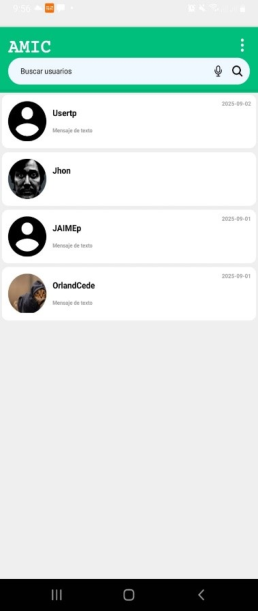
\includegraphics[width=0.18\linewidth]{1}
	\hfill
	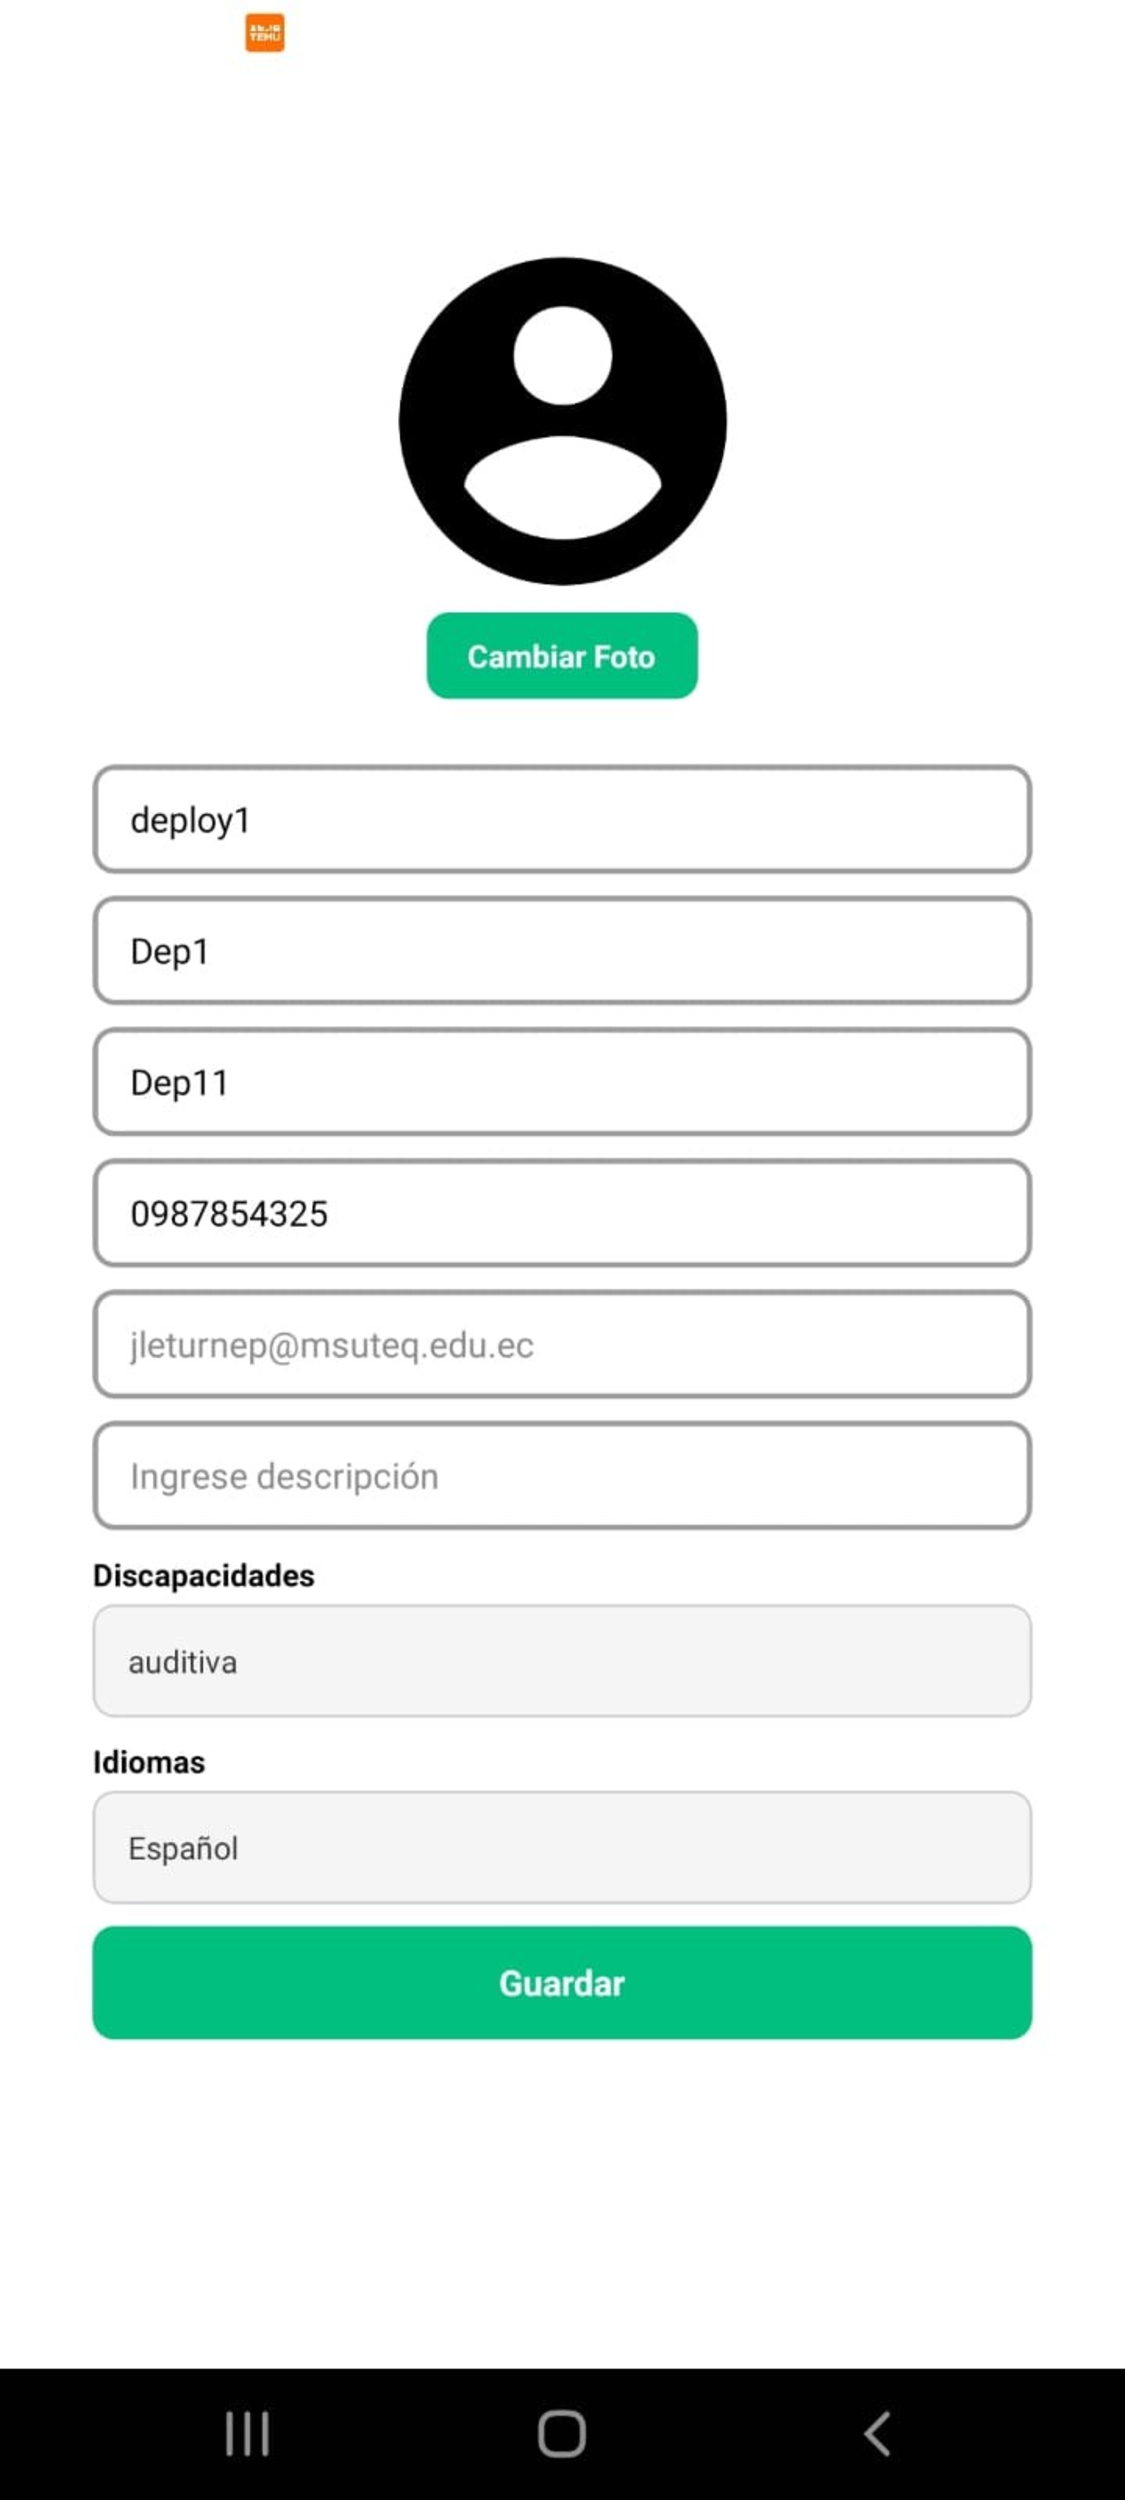
\includegraphics[width=0.18\linewidth]{2}
	\hfill
	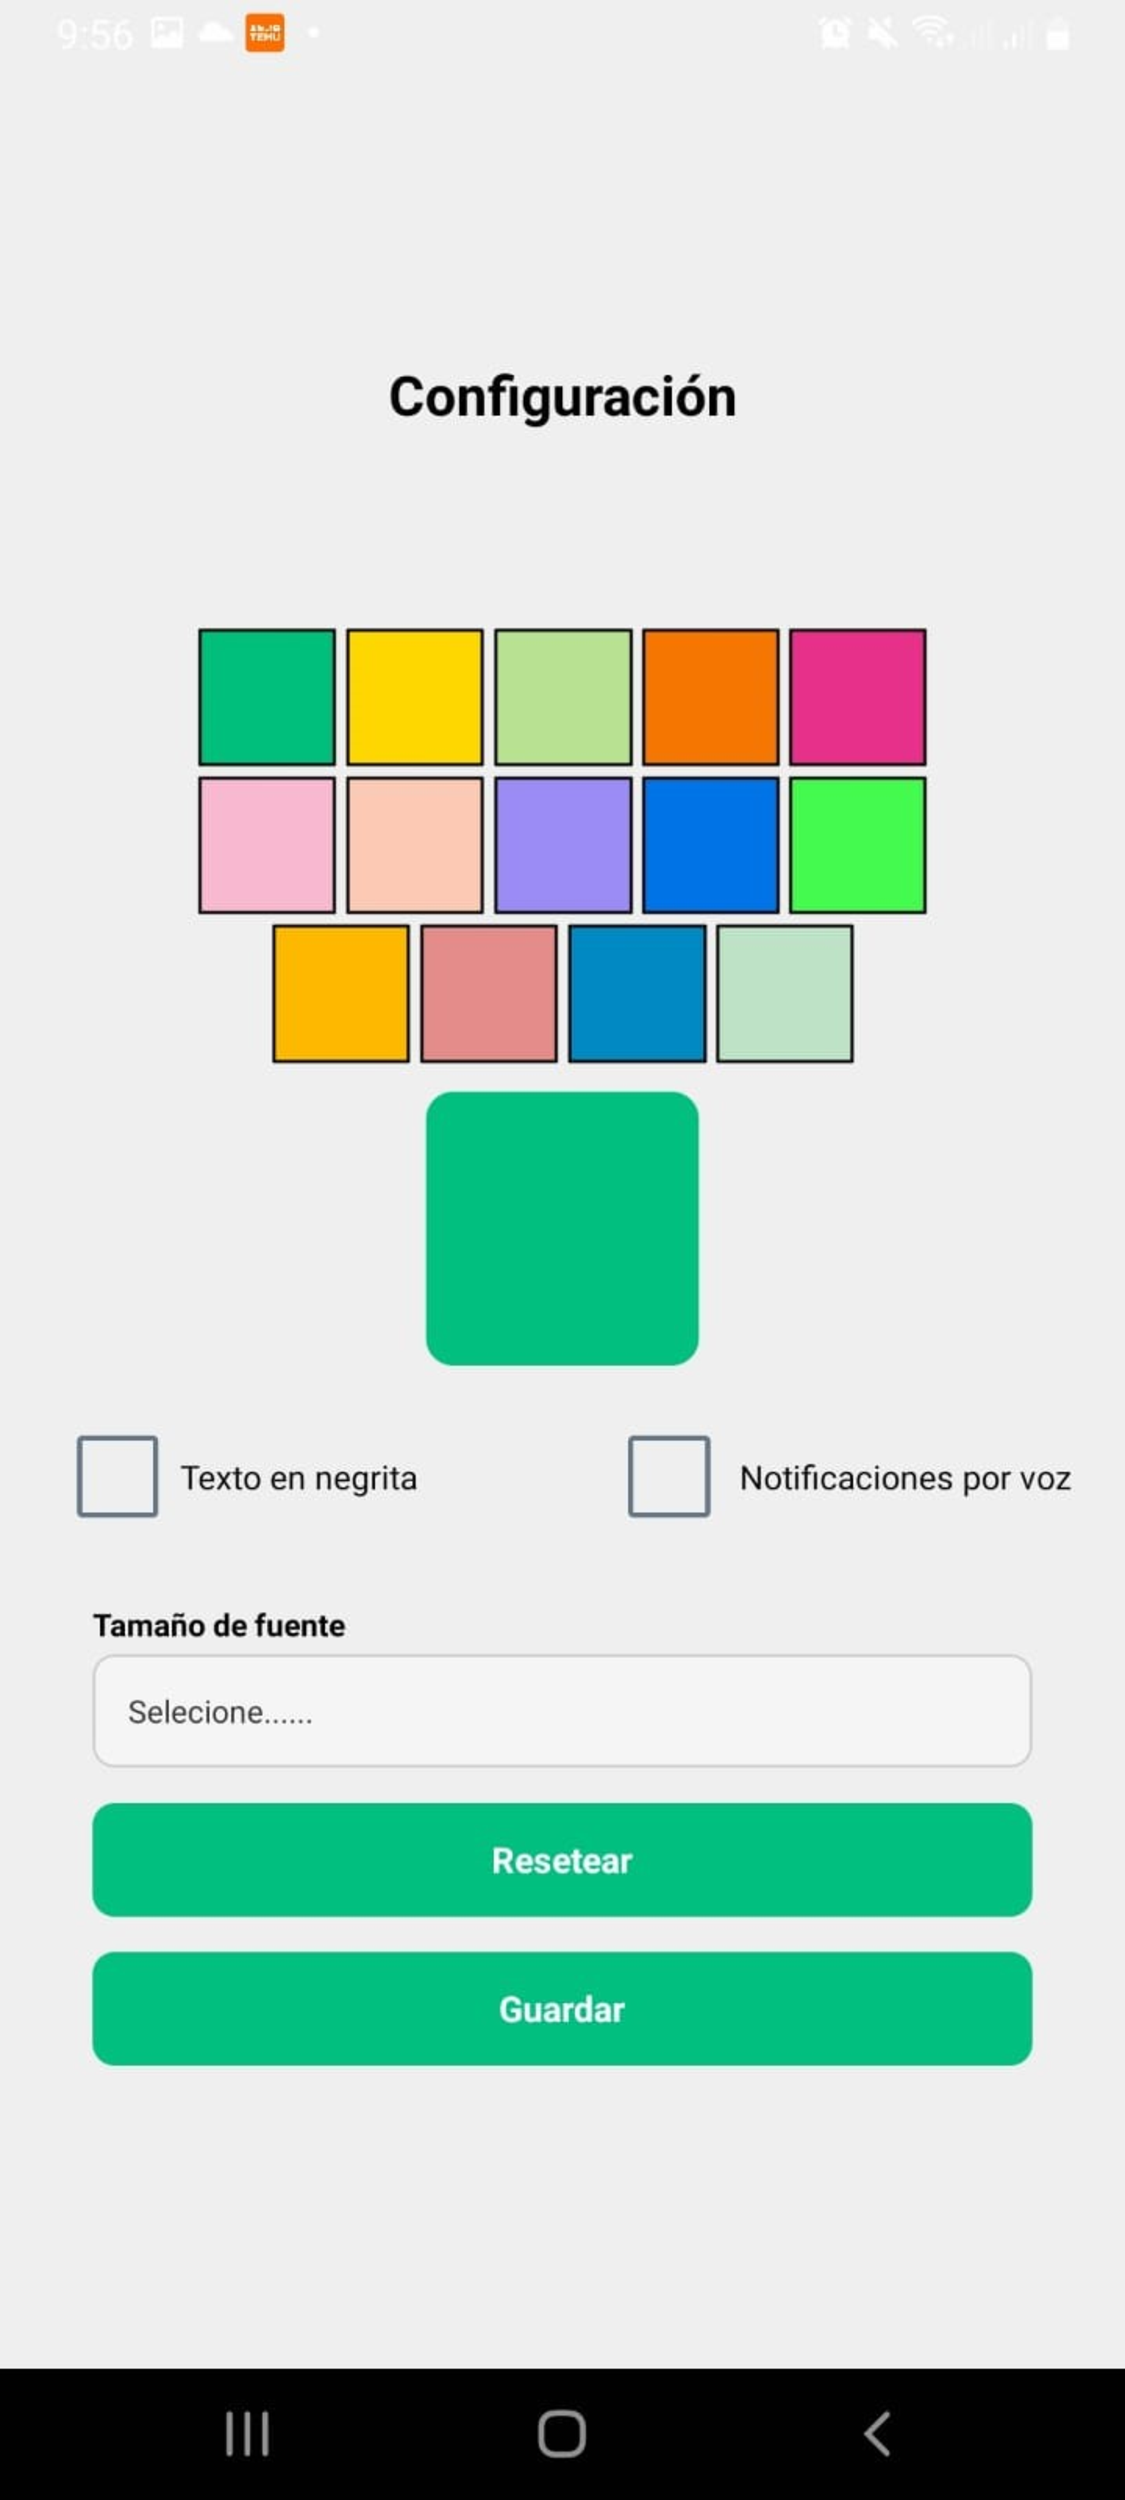
\includegraphics[width=0.18\linewidth]{3}
	\hfill
	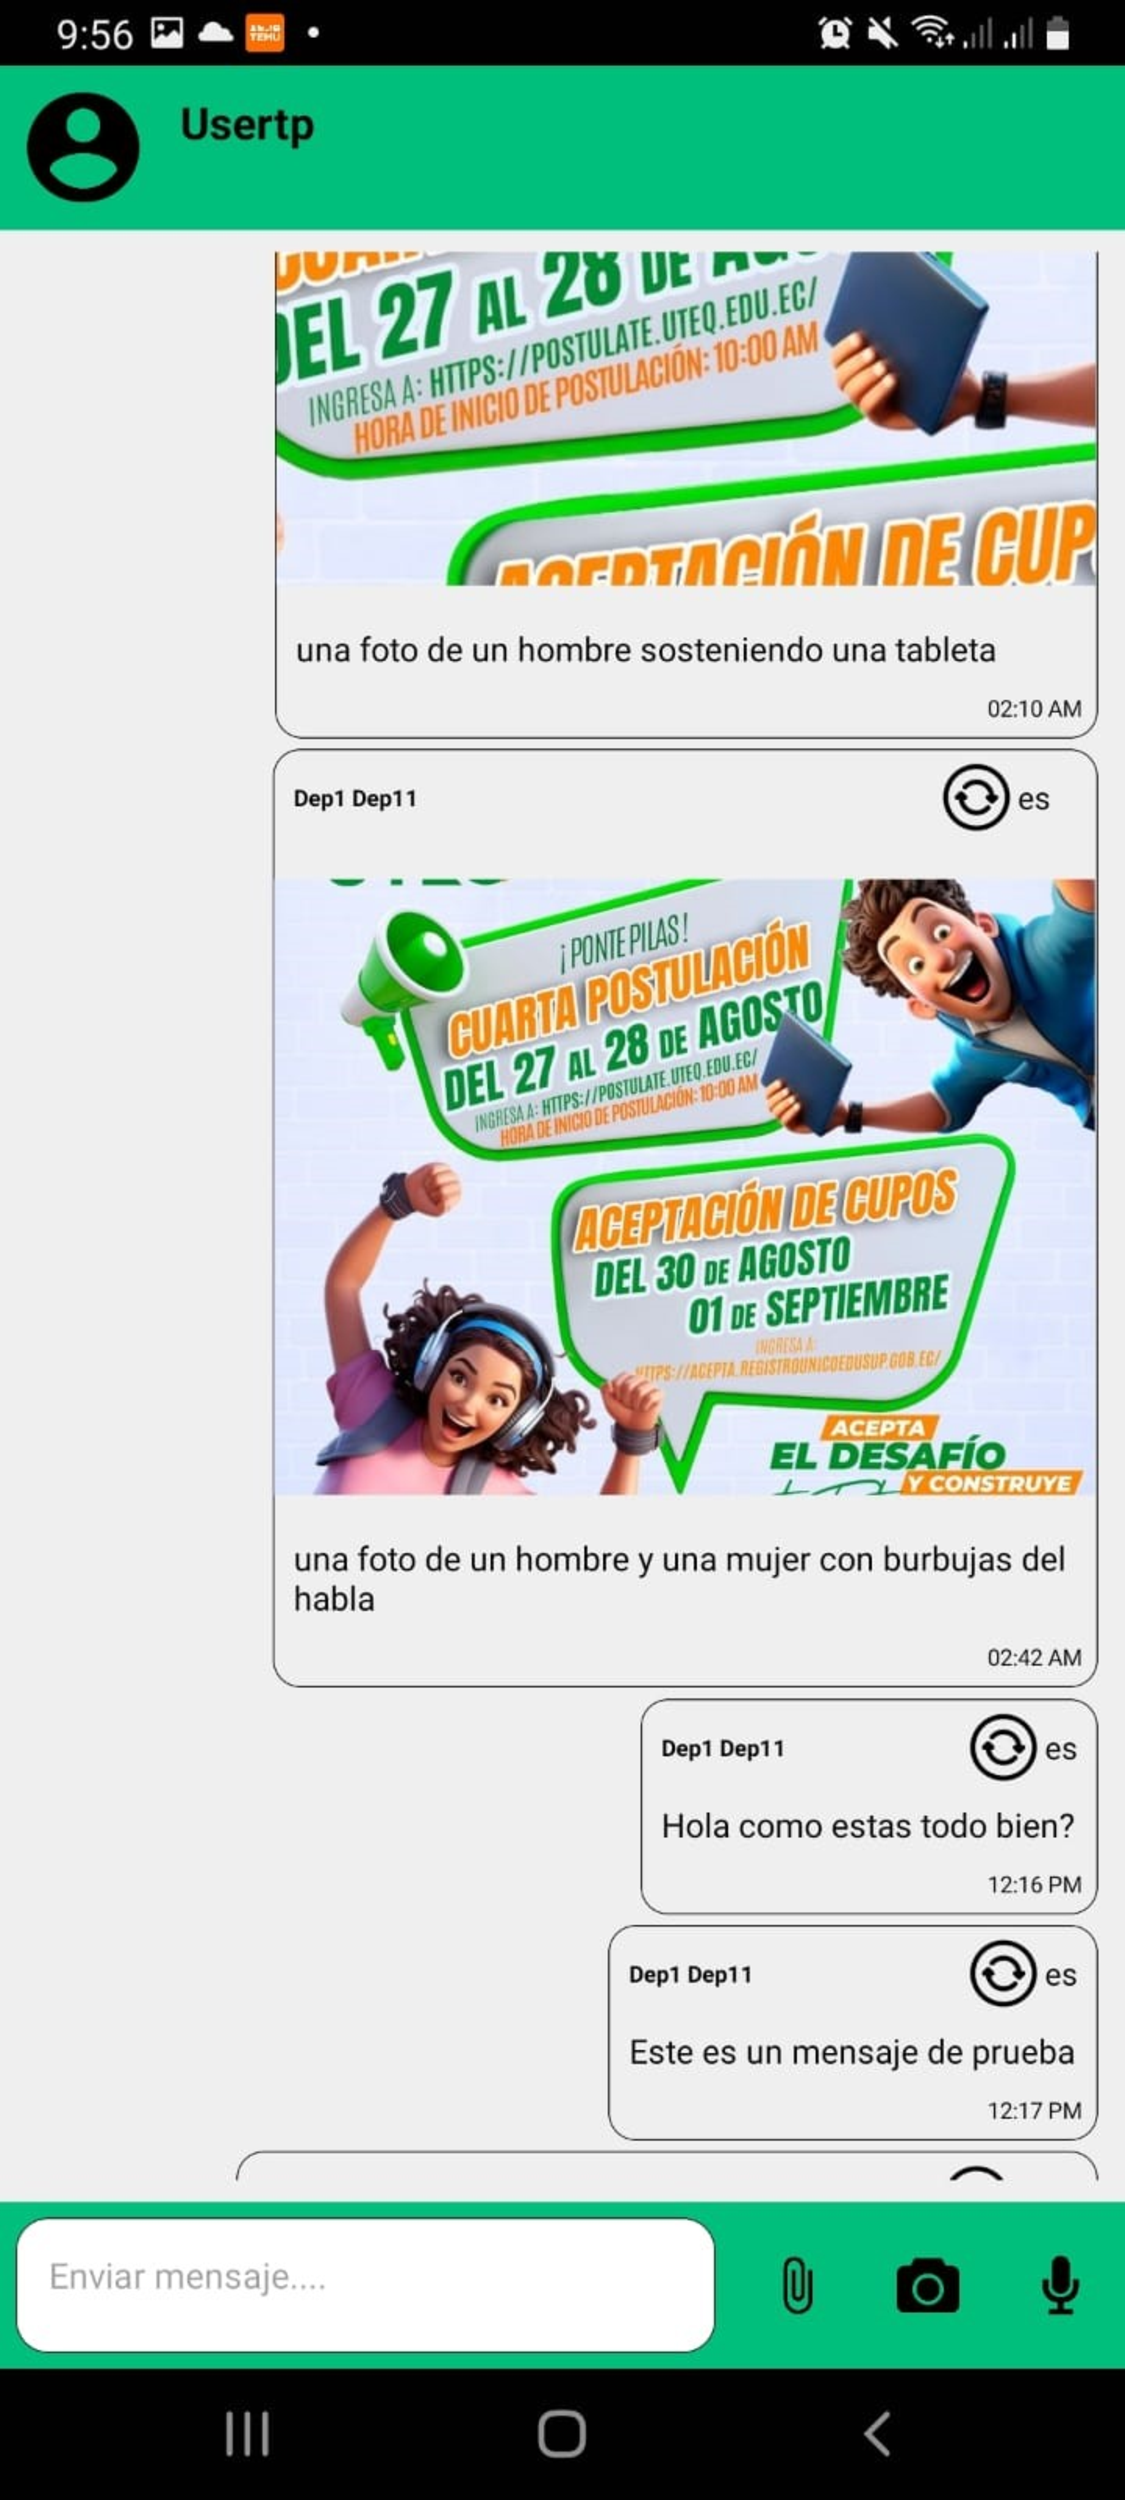
\includegraphics[width=0.18\linewidth]{4}
	\hfill
	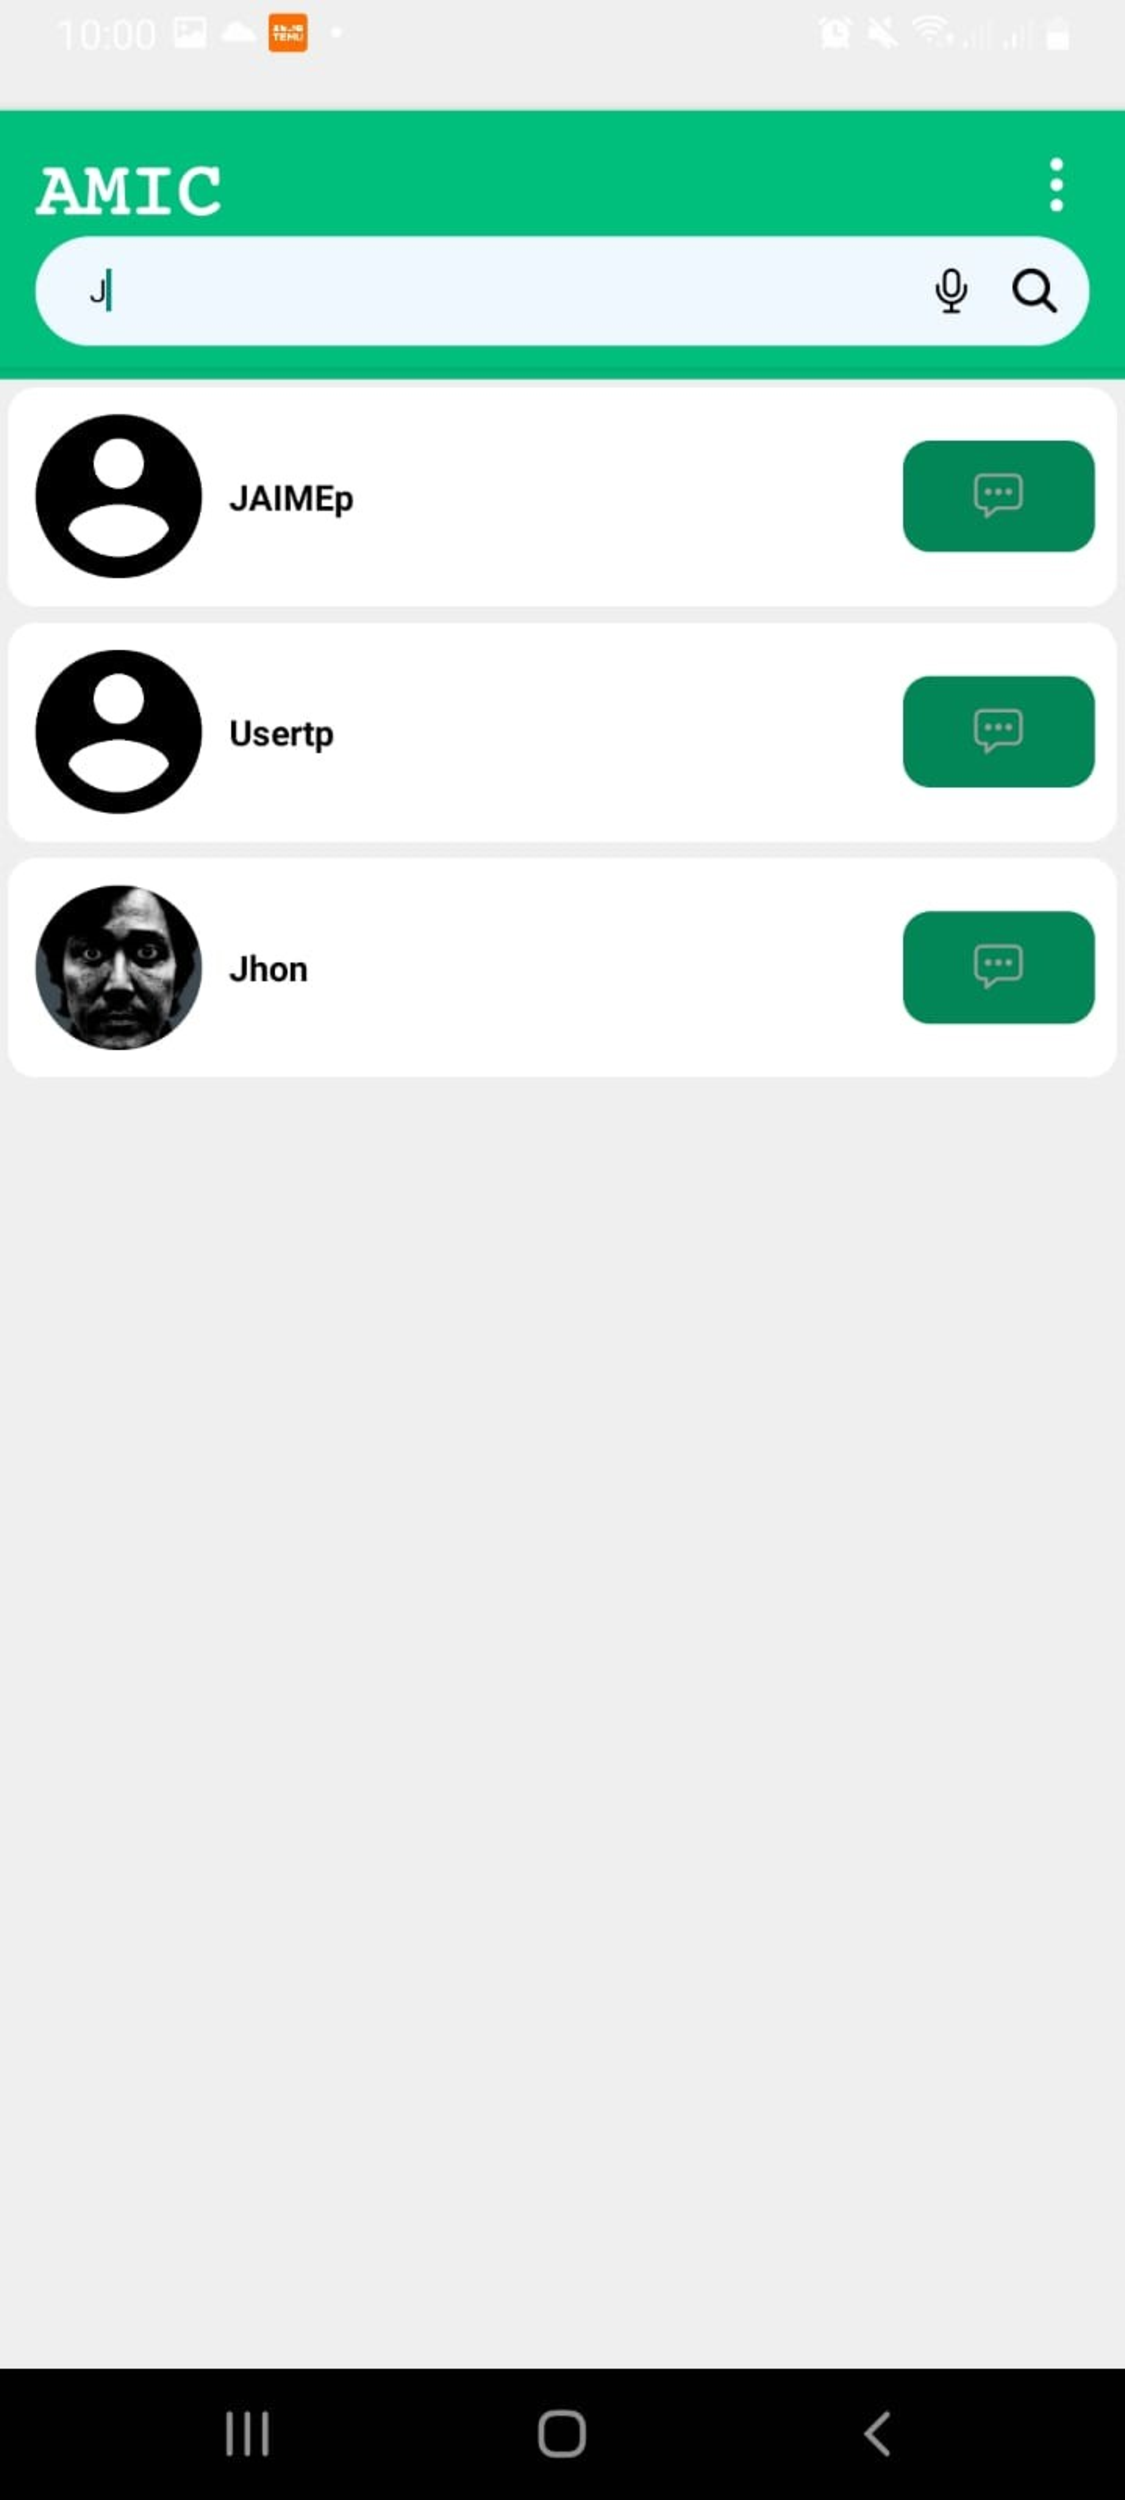
\includegraphics[width=0.18\linewidth]{5}
	\caption{Interfaces de la aplicación móvil}
	\label{fig:grupo_5_imagenes}
\end{figure}

\subsection {Evaluación de entregables}

\noindent En esta sección se presenta la evaluación de los entregables del proyecto, incluyendo la aplicación móvil y la documentación asociada. Todos los componentes y tareas planificadas fueron finalizados según el cronograma, cumpliendo con los objetivos y criterios de calidad establecidos, lo que garantiza la correcta implementación y disponibilidad del sistema. En la Tabla 33 se presentan los entregables que recibe el cliente del proyecto. La Tabla 34 muestra los componentes técnicos del sistema, mientras que la Tabla 35 detalla las tareas diarias realizadas para construir dichos componentes y generar los entregables.

\paragraph{Entregables}


\begin{itemize}
	\item \textbf{Aplicacion movil}: Aplicacion movil de mensajeria con conversion automatica de mensajes en tiempo real.
	\item \textbf{Documentacion}: Documentacion de todo el proceso de construccion del software.
\end{itemize}

\paragraph{Componentes}

\begin{itemize}
	\item \textbf{Interfaces móvil}: Pantallas y menú de la aplicación móvil
	\item \textbf{Funcionalidades móviles}: Configuración de comunicación de envío de mensaje, registro
	\item \textbf{Base de datos}: Sistema de almacenamiento estructurado donde se guardan todos los datos esenciales de la aplicación de mensajería
	\item \textbf{API de mensajería funcionando (Backend)}: API de procesamiento de datos de usuarios y de mensajes
	\item \textbf{API de conversión de mensajes}: API de inteligencia artificial que procesa los mensajes y los transforma según los requerimientos de los usuarios
	\item \textbf{Despliegue}: Configuración para instalar backend, frontend (generación de apk) y configurar servidores
	\item \textbf{Arquitectura del sistema}: Se define la arquitectura del sistema, es decir, se realiza un diagrama general dando a conocer cual son las diferentes secciones del sistema y como se están comunicando
	\item \textbf{Diagramas UML}: UML de Base de datos, Estado, Actividad, despliegue y casos de uso de la app
	\item \textbf{Documentación técnica de los componentes del sistema}: Descripción de la estructura de la base de datos, arquitectura del sistema, seguridad y las constantes integraciones realizadas
\end{itemize}

\paragraph{Tareas}

\begin{itemize}
	\item \textbf{Pantalla de registro}: Permite a los usuarios crear una cuenta y registrarse en la app.
	\item \textbf{Pantalla de perfil de usuario}: Muestra y permite editar la información personal del usuario.
	\item \textbf{Pantalla de configuración}: Permite ajustar preferencias de la app como colores, notificaciones por voz, tamaño de texto o discapacidad.
	\item \textbf{Pantalla principal de usuarios}: Muestra contactos para iniciar chats.
	\item \textbf{Pantalla de chat de usuarios}: Permite enviar y recibir mensajes en tiempo real con otros usuarios.
	\item \textbf{Pantalla de imágenes y video}: Permite previsualizar un video o imagenes.
	\item \textbf{Registro de usuarios}: Permite crear cuenta nueva en la aplicación.
	\item \textbf{Obtención de datos de usuarios}: Recupera información del perfil y contactos de los usuarios.
	\item \textbf{Obtención de chats}: Información de los chats amigos del usuario.
	\item \textbf{Envio de mensajes}: Permite enviar mensajes de texto y multimedia entre usuarios.
	\item \textbf{Cifrado de mensajes}: Protege la información de los mensajes durante la transmisión.
	\item \textbf{Configuración HTTP y WebSocket}: Gestiona la comunicación entre cliente y servidor en tiempo real.
	\item \textbf{Manejo de archivos}: Administra la creación, eliminación y actualización de archivos.
	\item \textbf{Grabar de audio}: Permite capturar mensajes de voz directamente desde la app.
	\item \textbf{Grabar video}: Permite grabar videos para enviar a otros usuarios.
	\item \textbf{Tomar foto en tiempo real}: Permite capturar imágenes con la cámara de forma instantánea para compartir.
	\item \textbf{Creación de funciones en la base de datos}: Implementa lógica dentro de las funciones para la obtención de datos.
	\item \textbf{Creación de modelos, servicios y repositorio}: Define la estructura de base de datos y la lógica de negocio en el backend.
	\item \textbf{Configuración de endpoints}: Establece rutas de la API para la comunicación entre cliente y servidor.
	\item \textbf{Configuración de WebSocket}: Habilita la mensajería en tiempo real entre usuarios.
	\item \textbf{Configuración y instalación del broker}: Implementa el sistema de mensajería que gestiona la comunicación en tiempo real (mensajes persistentes).
	\item \textbf{Comunicación con la API de conversión}: Conecta con API de conversión para transformar o procesar datos.
	\item \textbf{Cifrado de datos}: Protege la información sensible durante el almacenamiento y transmisión mediante el algoritmo AES.
	\item \textbf{Manejo de archivos}: Administra la creación, eliminación y actualización de archivos.
	\item \textbf{Configuración de carga de modelos}: Prepara e integra modelos de IA para su uso dentro de la aplicación.
	\item \textbf{Función TTS (Text To Speech)}: Convierte texto escrito en audio hablado.
	\item \textbf{Función STT (Speech To Text)}: Transcribe el audio en texto de forma automática.
	\item \textbf{Función de descripción de imagenes}: Genera texto descriptivo a partir de una imagen.
	\item \textbf{Función de procesamiento de videos}: Analiza o transforma contenido en video en subtitulos.
	\item \textbf{Manejo de archivos}: Administra la creación, eliminación y actualización de archivos.
	\item \textbf{Configuración del Docker}: Prepara contenedores para desplegar y ejecutar los servicios de la aplicación de forma aislada y portable.
	\item \textbf{Configuración del Nginx y SSL}: Establece el servidor web y proxy inverso para gestionar peticiones y seguridad SSL.
	\item \textbf{Configuración del servidor Window Server (EC2)}: Ajusta la infraestructura en la nube para hospedar y ejecutar la aplicación.
	\item \textbf{Generación del APK}: Compila la aplicación móvil en un archivo instalable para dispositivos Android.
	\item \textbf{Documentación de arquitectura del sistema}: Explica la estructura general y la interacción entre los componentes del sistema.
	\item \textbf{Mejoras de arquitectura}: Define optimizaciones en el desempeño del sistema.
	\item \textbf{Diagrama de Casos de uso}: Representa las interacciones entre los usuarios y el sistema.
	\item \textbf{Diagrama de actividades}: Muestra el flujo de procesos y decisiones dentro de la aplicación.
	\item \textbf{Diagrama de estados}: Describe los diferentes estados de un objeto y cómo cambia según eventos.
	\item \textbf{Diagrama de paquete}: Organiza los módulos del sistema en grupos lógicos.
	\item \textbf{Diagrama de base de datos}: Representa tablas, relaciones y estructuras de almacenamiento de datos.
	\item \textbf{Documentacion de las funcionalidades y pruebas}: Detalla cómo funcionan las características del sistema y los resultados de su validación.
	\item \textbf{Documentacion de investigaciones}: Registra la información teórica o técnica consultada que sustenta el desarrollo del sistema.
\end{itemize}

\subsection {Mantenimiento}

Dado que esta es una fase inicial del prototipo del sistema y que, hasta el momento, satisface las necesidades planteadas, esta etapa no se ha implementado. No obstante, se incluyen sugerencias de mantenimiento que podrían aplicarse en el futuro, tal como se muestran en la siguiente lista.

\begin{itemize}
	\item \textbf{Mejoras en la descripción de imágenes mediante la implementación de OCR}: Implementación de OCR para extraer texto de imágenes y generar descripciones automáticas, mejorando la accesibilidad y comprensión del contenido visual.
	
	\item \textbf{Mejora en la interacción con la aplicación móvil mediante comandos de voz}: Integración de control por voz para permitir a los usuarios navegar y ejecutar funciones de la aplicación de manera más eficiente.
	
	\item \textbf{Lectura de pantalla}: Funcionalidad que permite la lectura en voz alta del contenido de la aplicación, facilitando el acceso a personas con discapacidad visual y mejorando la experiencia de usuario.
	
	\item \textbf{Envío de mensajes entre grupos de usuarios}: Capacidad de crear grupos de usuarios dentro de la aplicación para enviar mensajes de manera simultánea, fomentando la comunicación en grupo más eficiente.
\end{itemize}


\section{Discusión}
\noindent Los resultados obtenidos en la etapa de accesibilidad de aplicaciones de mensajería muestran que aplicaciones como WhatsApp, Instagram y Messenger están un poco más avanzadas en cuanto a la accesibilidad para el usuario, mientras que aplicaciones como Telegram aún presentan limitaciones en sus funciones accesibles \cite{telegram2025}. 

\noindent Por otro lado, en las especificaciones de las APIs de inteligencia artificial que se están utilizando, existe una gran variedad. Algunas APIs ofrecen múltiples funcionalidades, como generación de texto y descripción de imágenes, lo que requiere un procesamiento más largo y costoso para los servidores donde se implementen. En cambio, existen modelos que se centran en una sola funcionalidad, por ejemplo, traducir texto o describir imágenes, y estos son más livianos en términos de procesamiento \cite{Varoquaux2025}.

\noindent Para la prevención de errores, principalmente se opta por la utilización de modelos locales livianos basados en una sola funcionalidad. Esto permite mantener velocidad y operatividad a largo plazo, ya que depender de una API en internet podría generar problemas si el servicio se cae \cite{Yugopuspito2024}.

\noindent En relación con la aceptabilidad de la aplicación, esta fue buena según los tres grupos de participantes, con una media cercana a 4 en las preguntas, y una tendencia mayor hacia la escala de 5. El 60 \% de los participantes tenía discapacidad visual, mientras que los participantes con discapacidad auditiva y las personas sin discapacidad representaron el 20 \% cada uno. A partir de esto, se identificó que la mayoría de los usuarios respondió entre las escalas 4 y 5. Sin embargo, algunas preguntas, como PTAM007, PTAM008, PTAM011 y PTAM012, mostraron una mediana de 3, más baja en comparación con las demás.

\noindent Los resultados de las pruebas de la aplicación muestran un rendimiento moderado en cuanto a aceptabilidad. Esto proporciona una base para discutir maneras de mejorar las funcionalidades de la aplicación y así apoyar de forma más efectiva a las personas que la necesitan para comunicarse.

\section{Conclusiones}

A partir de los resultados obtenidos en este proyecto de investigación, se pueden destacar las siguientes conclusiones:

\noindent Para conocer las principales limitaciones de accesibilidad, se realizó una revisión bibliográfica sobre las aplicaciones de mensajería más utilizadas, como WhatsApp, Telegram, Messenger e Instagram. A partir de ello, se describieron las funciones accesibles que ofrecen estas aplicaciones. Para analizar que funciones no cumplían este tipo de aplicaciones. Con base en las pautas de accesibilidad del W3C y las WCAG, se elaboró una lista de cotejo en la que se identificó cuáles de estas aplicaciones cumplen o no con ciertos criterios. observando que, aunque ya incluyen algunas funciones accesibles, todavía presentan limitaciones, especialmente en la lectura de mensajes y en el manejo general de la aplicación.

\noindent Para determinar qué inteligencias artificiales se utilizaron para la conversión de mensajes, se establecieron tres categorías: IAs de propósito general (con múltiples funciones como generación de texto o imágenes), IAs específicas (centradas en una sola tarea, como la conversión de audio a texto) y aquellas basadas en lenguajes de programación (librerías que usan modelos pequeños). Luego se elaboró una matriz con las funcionalidades de cada modelo y se definieron criterios para evaluar su desempeño, obteniendo que modelo tiene menos funcionalidades para una mayor rapidez de procesado. A partir de esto, se concluyó que tanto las IAs específicas como las librerías de programación resultan más óptimas para el procesamiento de recursos, ya que se enfocan en una sola tarea y no sobrecargan el sistema con funciones adicionales.

\noindent La interfaz de la aplicación se la desarrollo analizando las diferentes discapacidades que se está abordando con ello se especificaron diferentes idiomas en la cual tanto los textos, mensajes, notificaciones, y opciones del menú estan en idioma inglés y español. Con ello tambien cada una de las opciones se agregaron mensajes personalizados descriptivos con el fin de que el lector de pantalla del teléfono movil pueda leerlos sin problema. Tambien se tomó en cuenta el color y las opciones de toda la aplicación fueran claras y sin muchas opciones para garantizar la simplicidad de la misma y que fuera fácil usarla. 
\noindent La estructura de las funcionalidades inclusivas se definió mediante plantillas JSON, donde se especificaban los recursos requeridos para mensajes de texto, audio, video e imágenes. A partir de estas plantillas y con el uso de los modelos de IA seleccionados, se desarrollaron las distintas opciones de conversión, generando los recursos en inglés y español con su respectiva plantilla. Esto permite cambiar el idioma de los mensajes si el usuario lo necesita y, además, seleccionar el formato de visualización según la discapacidad, ya sea como audio o como texto.

\noindent Por lo tanto, AMIC es una aplicación de chat dirigida a personas con discapacidades visuales, auditivas y del habla. Ofrece la conversión de mensajes en tiempo real: el audio se transforma en texto o viceversa, y las imágenes enviadas se describen según la discapacidad y el idioma del usuario. Esto facilita la comunicación sin necesidad de acciones adicionales para interactuar con otros. Además, garantiza la seguridad de los mensajes mediante cifrado, lo que protege la privacidad y la información transmitida. También se realizaron pruebas de software, cuyos resultados fueron positivos, con un promedio de aceptación alto y una media superior a 3 en la mayoría de las preguntas del cuestionario.

\nocite{*}
\bibliographystyle{IEEEtran}
\bibliography{bellchatv2}


\end{document}


